% Options for packages loaded elsewhere
\PassOptionsToPackage{unicode}{hyperref}
\PassOptionsToPackage{hyphens}{url}
\documentclass[
]{article}
\usepackage{xcolor}
\usepackage[margin=1in]{geometry}
\usepackage{amsmath,amssymb}
\setcounter{secnumdepth}{5}
\usepackage{iftex}
\ifPDFTeX
  \usepackage[T1]{fontenc}
  \usepackage[utf8]{inputenc}
  \usepackage{textcomp} % provide euro and other symbols
\else % if luatex or xetex
  \usepackage{unicode-math} % this also loads fontspec
  \defaultfontfeatures{Scale=MatchLowercase}
  \defaultfontfeatures[\rmfamily]{Ligatures=TeX,Scale=1}
\fi
\usepackage{lmodern}
\ifPDFTeX\else
  % xetex/luatex font selection
\fi
% Use upquote if available, for straight quotes in verbatim environments
\IfFileExists{upquote.sty}{\usepackage{upquote}}{}
\IfFileExists{microtype.sty}{% use microtype if available
  \usepackage[]{microtype}
  \UseMicrotypeSet[protrusion]{basicmath} % disable protrusion for tt fonts
}{}
\makeatletter
\@ifundefined{KOMAClassName}{% if non-KOMA class
  \IfFileExists{parskip.sty}{%
    \usepackage{parskip}
  }{% else
    \setlength{\parindent}{0pt}
    \setlength{\parskip}{6pt plus 2pt minus 1pt}}
}{% if KOMA class
  \KOMAoptions{parskip=half}}
\makeatother
\usepackage{color}
\usepackage{fancyvrb}
\newcommand{\VerbBar}{|}
\newcommand{\VERB}{\Verb[commandchars=\\\{\}]}
\DefineVerbatimEnvironment{Highlighting}{Verbatim}{commandchars=\\\{\}}
% Add ',fontsize=\small' for more characters per line
\usepackage{framed}
\definecolor{shadecolor}{RGB}{248,248,248}
\newenvironment{Shaded}{\begin{snugshade}}{\end{snugshade}}
\newcommand{\AlertTok}[1]{\textcolor[rgb]{0.94,0.16,0.16}{#1}}
\newcommand{\AnnotationTok}[1]{\textcolor[rgb]{0.56,0.35,0.01}{\textbf{\textit{#1}}}}
\newcommand{\AttributeTok}[1]{\textcolor[rgb]{0.13,0.29,0.53}{#1}}
\newcommand{\BaseNTok}[1]{\textcolor[rgb]{0.00,0.00,0.81}{#1}}
\newcommand{\BuiltInTok}[1]{#1}
\newcommand{\CharTok}[1]{\textcolor[rgb]{0.31,0.60,0.02}{#1}}
\newcommand{\CommentTok}[1]{\textcolor[rgb]{0.56,0.35,0.01}{\textit{#1}}}
\newcommand{\CommentVarTok}[1]{\textcolor[rgb]{0.56,0.35,0.01}{\textbf{\textit{#1}}}}
\newcommand{\ConstantTok}[1]{\textcolor[rgb]{0.56,0.35,0.01}{#1}}
\newcommand{\ControlFlowTok}[1]{\textcolor[rgb]{0.13,0.29,0.53}{\textbf{#1}}}
\newcommand{\DataTypeTok}[1]{\textcolor[rgb]{0.13,0.29,0.53}{#1}}
\newcommand{\DecValTok}[1]{\textcolor[rgb]{0.00,0.00,0.81}{#1}}
\newcommand{\DocumentationTok}[1]{\textcolor[rgb]{0.56,0.35,0.01}{\textbf{\textit{#1}}}}
\newcommand{\ErrorTok}[1]{\textcolor[rgb]{0.64,0.00,0.00}{\textbf{#1}}}
\newcommand{\ExtensionTok}[1]{#1}
\newcommand{\FloatTok}[1]{\textcolor[rgb]{0.00,0.00,0.81}{#1}}
\newcommand{\FunctionTok}[1]{\textcolor[rgb]{0.13,0.29,0.53}{\textbf{#1}}}
\newcommand{\ImportTok}[1]{#1}
\newcommand{\InformationTok}[1]{\textcolor[rgb]{0.56,0.35,0.01}{\textbf{\textit{#1}}}}
\newcommand{\KeywordTok}[1]{\textcolor[rgb]{0.13,0.29,0.53}{\textbf{#1}}}
\newcommand{\NormalTok}[1]{#1}
\newcommand{\OperatorTok}[1]{\textcolor[rgb]{0.81,0.36,0.00}{\textbf{#1}}}
\newcommand{\OtherTok}[1]{\textcolor[rgb]{0.56,0.35,0.01}{#1}}
\newcommand{\PreprocessorTok}[1]{\textcolor[rgb]{0.56,0.35,0.01}{\textit{#1}}}
\newcommand{\RegionMarkerTok}[1]{#1}
\newcommand{\SpecialCharTok}[1]{\textcolor[rgb]{0.81,0.36,0.00}{\textbf{#1}}}
\newcommand{\SpecialStringTok}[1]{\textcolor[rgb]{0.31,0.60,0.02}{#1}}
\newcommand{\StringTok}[1]{\textcolor[rgb]{0.31,0.60,0.02}{#1}}
\newcommand{\VariableTok}[1]{\textcolor[rgb]{0.00,0.00,0.00}{#1}}
\newcommand{\VerbatimStringTok}[1]{\textcolor[rgb]{0.31,0.60,0.02}{#1}}
\newcommand{\WarningTok}[1]{\textcolor[rgb]{0.56,0.35,0.01}{\textbf{\textit{#1}}}}
\usepackage{longtable,booktabs,array}
\usepackage{calc} % for calculating minipage widths
% Correct order of tables after \paragraph or \subparagraph
\usepackage{etoolbox}
\makeatletter
\patchcmd\longtable{\par}{\if@noskipsec\mbox{}\fi\par}{}{}
\makeatother
% Allow footnotes in longtable head/foot
\IfFileExists{footnotehyper.sty}{\usepackage{footnotehyper}}{\usepackage{footnote}}
\makesavenoteenv{longtable}
\usepackage{graphicx}
\makeatletter
\newsavebox\pandoc@box
\newcommand*\pandocbounded[1]{% scales image to fit in text height/width
  \sbox\pandoc@box{#1}%
  \Gscale@div\@tempa{\textheight}{\dimexpr\ht\pandoc@box+\dp\pandoc@box\relax}%
  \Gscale@div\@tempb{\linewidth}{\wd\pandoc@box}%
  \ifdim\@tempb\p@<\@tempa\p@\let\@tempa\@tempb\fi% select the smaller of both
  \ifdim\@tempa\p@<\p@\scalebox{\@tempa}{\usebox\pandoc@box}%
  \else\usebox{\pandoc@box}%
  \fi%
}
% Set default figure placement to htbp
\def\fps@figure{htbp}
\makeatother
\ifLuaTeX
  \usepackage{luacolor}
  \usepackage[soul]{lua-ul}
\else
  \usepackage{soul}
\fi
% definitions for citeproc citations
\NewDocumentCommand\citeproctext{}{}
\NewDocumentCommand\citeproc{mm}{%
  \begingroup\def\citeproctext{#2}\cite{#1}\endgroup}
\makeatletter
 % allow citations to break across lines
 \let\@cite@ofmt\@firstofone
 % avoid brackets around text for \cite:
 \def\@biblabel#1{}
 \def\@cite#1#2{{#1\if@tempswa , #2\fi}}
\makeatother
\newlength{\cslhangindent}
\setlength{\cslhangindent}{1.5em}
\newlength{\csllabelwidth}
\setlength{\csllabelwidth}{3em}
\newenvironment{CSLReferences}[2] % #1 hanging-indent, #2 entry-spacing
 {\begin{list}{}{%
  \setlength{\itemindent}{0pt}
  \setlength{\leftmargin}{0pt}
  \setlength{\parsep}{0pt}
  % turn on hanging indent if param 1 is 1
  \ifodd #1
   \setlength{\leftmargin}{\cslhangindent}
   \setlength{\itemindent}{-1\cslhangindent}
  \fi
  % set entry spacing
  \setlength{\itemsep}{#2\baselineskip}}}
 {\end{list}}
\usepackage{calc}
\newcommand{\CSLBlock}[1]{\hfill\break\parbox[t]{\linewidth}{\strut\ignorespaces#1\strut}}
\newcommand{\CSLLeftMargin}[1]{\parbox[t]{\csllabelwidth}{\strut#1\strut}}
\newcommand{\CSLRightInline}[1]{\parbox[t]{\linewidth - \csllabelwidth}{\strut#1\strut}}
\newcommand{\CSLIndent}[1]{\hspace{\cslhangindent}#1}
\setlength{\emergencystretch}{3em} % prevent overfull lines
\providecommand{\tightlist}{%
  \setlength{\itemsep}{0pt}\setlength{\parskip}{0pt}}
\usepackage{tocloft}
\renewcommand{\cftsecfont}{\large}
\renewcommand{\cftsubsecfont}{\normalsize}
\renewcommand{\cftsecpagefont}{\normalsize}
\renewcommand{\cftsubsecpagefont}{\normalsize}
\setlength{\cftbeforesecskip}{0pt}
\setlength{\cftbeforesubsecskip}{0pt}
\setcounter{secnumdepth}{3}
\setcounter{tocdepth}{4}
\usepackage{titling}
\setlength{\droptitle}{-3em}
\setlength{\parindent}{0pt}
\setlength{\parskip}{1em}
\setlength{\cftbeforetoctitleskip}{-2em}
\usepackage{fancyhdr}
\usepackage{lastpage}
\usepackage{float}
\usepackage{placeins}
\usepackage{setspace}
\setstretch{1.5}

% 1️⃣ Title Page: No numbering (COMPLETELY HIDDEN)
\pagenumbering{gobble}  % Disable page numbering completely
\pagestyle{empty}  % No header or footer
\thispagestyle{empty}  % Ensure this page stays empty

% 2️⃣ Roman numeral pages (Abstract, TOC, List of Figures/Tables)
\newpage
\pagenumbering{roman}  % Start Roman numerals
\fancypagestyle{roman}{
  \fancyhf{}  % Clear all headers and footers
  \renewcommand{\headrulewidth}{0pt}  % No header line
  \fancyfoot[C]{\thepage}  % ONLY show the page number (ii, iii, iv)
}
\pagestyle{roman}  % Apply to all Roman numeral pages
\thispagestyle{roman}  % Ensure it applies immediately

% 🔹 Ensure TOC, List of Figures/Tables KEEP the correct Roman numeral format
\renewcommand{\tableofcontents}{
  \newpage
  \pagenumbering{roman} % Ensure Roman numerals
  \pagestyle{roman} % Keep TOC in Roman style
  \thispagestyle{roman} % Apply immediately
  \begingroup
  \let\cleardoublepage\clearpage % Prevent unwanted blank pages
  \toccontents
  \endgroup
}

\renewcommand{\listoffigures}{
  \newpage
  \pagenumbering{roman} % Ensure Roman numerals
  \pagestyle{roman} % Keep style consistent across pages
  \thispagestyle{roman} % Apply immediately
  \begingroup
  \let\cleardoublepage\clearpage % Prevent unwanted blank pages
  \lofcontents
  \endgroup
}

\renewcommand{\listoftables}{
  \newpage
  \pagenumbering{roman} % Ensure Roman numerals
  \pagestyle{roman} % Keep style consistent across pages
  \thispagestyle{roman} % Apply immediately
  \begingroup
  \let\cleardoublepage\clearpage % Prevent unwanted blank pages
  \lotcontents
  \endgroup
}

% 3️⃣ Arabic numeral pages (Main content starts here)
\newpage
\pagenumbering{arabic}  % Start Arabic numbering
\pagestyle{plain} % Reset to simple style before applying fancy
\thispagestyle{plain} % Apply immediately

% Apply "Page X of Y" format for Arabic pages
\fancypagestyle{arabic}{
  \fancyhf{}  % Clear headers/footers
  \renewcommand{\headrulewidth}{0pt}  % No header
  \fancyfoot[C]{Page \thepage\ of \pageref{LastPage}} % Show "Page X of Y"
}
\pagestyle{arabic} % Apply globally for main content
\thispagestyle{arabic} % Ensure it applies immediately on the first Arabic page

\usepackage{booktabs}
\usepackage{longtable}
\usepackage{array}
\usepackage{multirow}
\usepackage{wrapfig}
\usepackage{float}
\usepackage{colortbl}
\usepackage{pdflscape}
\usepackage{tabu}
\usepackage{threeparttable}
\usepackage{threeparttablex}
\usepackage[normalem]{ulem}
\usepackage{makecell}
\usepackage{xcolor}
\usepackage{bookmark}
\IfFileExists{xurl.sty}{\usepackage{xurl}}{} % add URL line breaks if available
\urlstyle{same}
\hypersetup{
  hidelinks,
  pdfcreator={LaTeX via pandoc}}

\author{}
\date{\vspace{-2.5em}}

\begin{document}

\pagenumbering{gobble} % Completely disable numbering on title page
\thispagestyle{empty} % Ensure first page has no header/footer
\centering
\LARGE

\textbf{Opting Out: Cryptocurrency Under Consideration of Currency Substitution}

\large

Master Thesis

\large

Alec Vayloyan, MSc Student Applied Information and Data Science

\large

Submission for 16.05.2025


\includegraphics[width=3in]{cover.png} \large

Supervisor: Dr.~Denis Bieri (\href{mailto:denis.bieri@hslu.ch}{\nolinkurl{denis.bieri@hslu.ch}})

Co-Supervisor: Dr.~Thomas Ankenbrand (\href{mailto:thomas.ankenbrand@hslu.ch}{\nolinkurl{thomas.ankenbrand@hslu.ch}})

E-Mail Author: \href{mailto:vayloyanalec49@gmail.com}{\nolinkurl{vayloyanalec49@gmail.com}}

Thesis submitted in partial requirement for a Master's degree in Applied Information and Data Science at the Lucerne University of Applied Science

Spring Semester 2025 \vspace{2cm}

\begin{flushleft}


\includegraphics[width=2.5in]{hslu_logo.png}

\end{flushleft}
\pagenumbering{roman}
\pagestyle{roman}
\newpage

\LARGE

\begin{center}

\Large

\textbf{Abstract}

\end{center}

\normalsize

We analyze the drivers behind this shift, including trust in traditional banking, regulatory landscapes, and the increasing adoption of blockchain technology. Using a combination of quantitative data analysis and qualitative insights, we examine whether Bitcoin and other cryptocurrencies serve as viable alternatives to government-issued money. The study also investigates the risks associated with cryptocurrency-based economies, including price volatility, regulatory uncertainty, and financial exclusion, this is a fake abstract placeholder.

\vspace{8cm}

\raggedright

\textbf{Keywords:} Cryptocurrency, Currency Substitution, Dollarization 2.0, Bitcoin

\newpage

\tableofcontents

\newpage

\listoffigures

\clearpage

\listoftables

\newpage

\pagenumbering{arabic}
\pagestyle{arabic}

\section{Motivation and Topic Definition}\label{motivation-and-topic-definition}

The development of cryptocurrencies, spawned alongside blockchain technology, have challenged traditional monetary systems and economic structures. Since its inception in the wake of the Global Financial Crisis, cryptocurrencies and particularily Bitcoin have been championed by advocates for its decentralized nature, security, and potential as a replacement for fiat currencies. Cryptocurrencies are often viewed as a solution for individuals and nations where conventional financial systems are dysfunctional or highly volatile, providing an alternative currency that is not controlled by the same rules as a potentially dysfunctional monetary system.

\subsection{``Traditional'' Cryptocurrencies}\label{traditional-cryptocurrencies}

In contrast to fiat currencies, which derive their value from governmental decree and are backed by legal frameworks, traditional cryptocurrencies operate on a decentralized network of peer-to-peer transactions that do not rely on a central authority. This decentralized nature means that transactions are verified by a distributed ledger known as blockchain, rather than by a trusted intermediary like a bank. Some cryptocurrencies, most notably Bitcoin have a function which reduces and eventually ceases the issuance of new coins through network design. This theoretically deflationary approach is in stark contrast to fiat currencies, where the authorities issuing target an inflation rate of 2\% annually Central Bank News (\citeproc{ref-centralbanknews2025}{2025}). The slow(ing) growth in supply of Bitcoin relative to the existing stock of coins is what leads to idea that Bitcoin is ``Digital Gold'', since the stability in value of gold is attributable to the same phenomenon of large existing stocks with very slow growth in supply (\citeproc{ref-ammousBTCstd}{Ammous, 2018b}). The lack of control by a single entity and slow growth have spawned the belief that cryptocurrencies are immune to inflationary pressures, government control, and political instability, which can all negatively affect those using fiat currencies in the \emph{status quo} financial system.

\subsection{Stablecoins}\label{stablecoins}

An important subset of cryptocurrencies in relation to this topic are stablecoins. These are cryptocurrencies which have prices linked to reference assets. In this sense, they are different to ``traditional'' cryptocurrencies in that the price is driven by centralized actors, rather than the collective decicions of the users. Catalini et al. (\citeproc{ref-catalini2022}{2022}) identifies the main ways stability can be achieved are:

\begin{enumerate}
\def\labelenumi{\arabic{enumi}.}
\item
  Backing of the stablecoins by one or more fiat currencies.
\item
  Backing of the stablecoin by one or more cryptocurrencies, not issued by the same entity as the stablecoin.
\item
  Backing of the stablecoin by one or more cryptocurrency issued by the same entity as the stablecoin, which can be used to manipulate the price of the stablecoin (algorithmic stablecoins).
\item
  Additionally, some research has found that the increased purchase of stablecoins during market downturns, rather than traditional cryptocurrencies acts as an additional stabilizing force for stablecoins, beyond the currency architecture (\citeproc{ref-baur2021}{Baur \& Hoang, 2021}; \citeproc{ref-lyons2020}{Lyons \& Viswanath-Natraj, 2020}).
\end{enumerate}

Stablecoins have the potential to combine the stability benefits of well managed fiat currencies with the settlement speed advantages of cryptocurrencies(\citeproc{ref-catalini2022}{Catalini et al., 2022}). And while the consensus is that stablecoins are more stable than traditional cryptocurrencies, they have not managed to maintain the desired pegs to fiat currencies consistently (\citeproc{ref-baughman2022}{Baughman et al., 2022}; \citeproc{ref-kosse2023}{Kosse et al., 2023}).

\subsection{Adoption of Cryptocurrencies}\label{adoption-of-cryptocurrencies}

Cryptocurrency adoption has not been uniform. As Figure \ref{fig:AdoptionMap} shows, for those countries with available data, the number of survey respondents who said they use cryptocurrency was as low as 6\% and as high as 47\%. That is a considerable difference! Factors driving cryptocurrency adoption vary greatly across regions and are often context-specific, such as inflationary pressures, technological accessibility, and government regulations. Understanding the global drivers of cryptocurrency adoption, particularly in the context of factors that are more relevant for emerging markets with less developed financial regulations provides a valuable insight into cryptocurrencies potential future size and role in the global economy.

\FloatBarrier

\begin{figure}
\centering
\pandocbounded{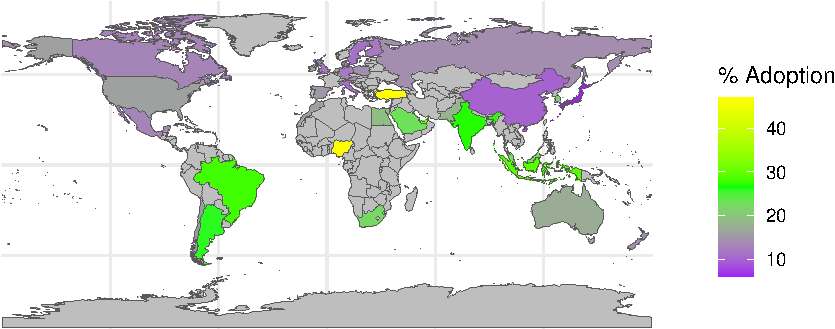
\includegraphics[keepaspectratio]{Thesis-Vayloyan6_files/figure-latex/AdoptionMap-1.pdf}}
\caption{\label{fig:AdoptionMap}WorldMap Showing Cryptocurrency Adoption Percentage for 2023 (Statista, 2024a)}
\end{figure}

\FloatBarrier

In parallel, a vast body of literature exists around the concept of \emph{currency substitution}, where individuals in a country predominately use foreign currencies, rather than their local currencies for the functions of money (\citeproc{ref-calvo2002}{Calvo, 2002}). The fundemental drivers behind currency substitution and touted benefits of cryptocurrencies are in many ways similar, with individuals often turning to foreign currencies or decentralized alternatives when local currencies fail to serve them.

This research draws upon the well-established theories of currency substitution to explore the factors driving cryptocurrency adoption. By examining the similarities between currency substitution and cryptocurrency adoption, this study aims to determine whether the predictors of currency substitution can be built into models of cryptocurrency adoption to improve the explanatory power.

\subsection{Literature Gap and Relevance}\label{literature-gap-and-relevance}

The research is relevant for both academics and policymakers. The contribution to the academic literature is twofold. Firstly, existing models cannot fully explain the differences in adoption seen across countries. Secondly and more innovativley, the paper provides corresponding analysis for cryptocurrency through the lens of currency substitution, which has not been done before to the best of knowledge. As will be seen in the section \hyperref[dependent-variable-bitcoin-adoption]{Dependent Variable: Bitcoin Adoption} this research makes use of a new and to my knowledge previously not studied panel dataset of Bitcoin adoption that will be able to capture the most recent trends in this area.

In terms of policymakers, it is important for them to be able to understand how changes in underlying economic conditions may influence the use of cryptocurrency as this will have policy implications. It is likely that questions around cryptocurrency will increase in importance in the future due to the increased interest and usage of cryptocurrencies globally: Both from private individuals and governments looking to capitalize on the technology in various ways. Figure \ref{fig:fig-btc} below shows the trend in cryptocurrency's market capitalization in USD from 2010 - 2025. This increased capitalization is evidence of interest in the technology among investors.

\FloatBarrier

\begin{figure}
\centering
\pandocbounded{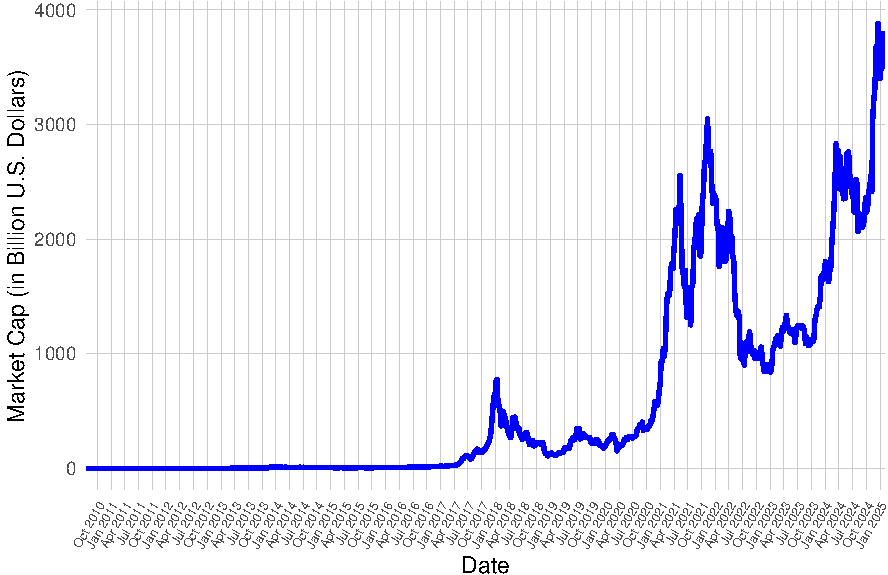
\includegraphics[keepaspectratio]{Thesis-Vayloyan6_files/figure-latex/fig-btc-1.pdf}}
\caption{\label{fig:fig-btc}Cryptocurrency Market Capitalization 2010-2025 (Statista, 2025)}
\end{figure}

\FloatBarrier

In addition to the increased capitalization, policymakers have begun to carve out a space for blockchain technology in their economies in different ways. Likely the most famous example is El Salvador legislating Bitcoin as a legal tender in their country in 2021 (\citeproc{ref-bbc2021}{BBC, 2021}). However there are also other examples such as Canton Zug in Switzerland allowing residents to pay taxes up to CHF 1.5M with certain cryptocurrencies or several large institutional investors and sovereign wealth funds globally purchasing Bitcoin (\citeproc{ref-chainalysis2024}{Chainalysis, 2024}; \citeproc{ref-kantonzug}{Kanton Zug, n.d.}). At the time of writing, a recent example is Mubadala Investment's (Abu Dhabi) purchase of USD 436M in Bitcoin (\citeproc{ref-cryptodaily2025}{Cryptodaily, 2025}). All of that is to say, research aiming to understand drivers of cryptocurrency demand is likely to remain or increase in relevance in the foreseeable future.

\subsection{Decentralized Alternatives}\label{decentralized-alternatives}

As alluded to earlier cryptocurrencies have been suggested as the alternative to dysfunctional currencies. There are two key reasons for this: the internet-based nature and relative price stability.

Firstly, the internet based nature means that most people with a smartphone and internet can relatively easily access the necessary infrastructure to buy and sell cryptocurrencies. This extends beyond political borders - there is nothing intrinsically hindering people or institutions in different political jurisdictions from exchanging with each other. This is different to using fiat currencies, where financial institutions (usually) comply with regulations on the transfer of digital funds and the lack of physical proximity between buyers and sellers fiat currency limits the ability to exchange cash.

Secondly, depending on the inflationary context, the price of cryptocurrencies can be relatively stable. Stability of a local currency is usually measured either against inflation or a exchange rate to a major currency. The price fluctuations of particularily stablecoins can be lower than those of many fiat currencies, and even Bitcoin, which has no intrinsic stability mechanisms has maintained it's value against fiat currencies in high inflation settings.

The use of alternative currencies by people is not new, there is an entire body of research devoted to this practice, known as \emph{currency substitution}. Currency substitution is defined by Calvo (\citeproc{ref-calvo2002}{2002}) as the highly prevalent use of \ul{foreign} fiat currencies to fulfill any of the three functions of money (store of value, means of exchange, unit of account). Note, there is also something known as \emph{official currency substitution}, which is when a government officially adopts a foreign currency as a legal tender in their own country. However, this paper refers to the personal and in unofficial use by individuals.

\textbf{Roadmap}

For the definition of the research topic, two questions / fields are of interest: ``What drives currency substitution?'' and ``What drives the adoption of cryptocurrencies?'' These topics will not be investigated in separate literature reviews in the next section. From these reviews the research question ``{[}\ul{RQ HERE}{]} will be developed. Next, the methods, data and data transformation used to answer the research question will be discussed and visualized. Finally, the statistical results are shown, discussed and placed in the academic context to provide conclusions for researchers and policymakers interested in what factors can drive the adoption of cryptocurrency.

\newpage

\section{Literature Review: Currency Substitution}\label{literature-review-currency-substitution}

There is a body of academic literature evaluating why individuals use cryptocurrency, this section discusses this literature. Those interested in a succinct visual overview should visit Appendix 1, subsection: \hyperref[literature-area-1-drivers-of-currency-substitution]{Literature Area 1: Drivers of Currency Substitution}.

\subsection{Currency Stability}\label{currency-stability}

The stability of currencies as a driver for cryptocurrency adoption is a debated issue in the academic literature, since there are two main ways of looking at currency stability (Inflation and Exchange Rate), these topics are evaluated separate.

\subsubsection{Inflation}\label{inflation}

Both perceived and real economic problems are identified in the literature as reasons for people to engaging in currency substitution, the primary economic issue here is inflation. There are quantitative studies, such as those by Vieira et al. (\citeproc{ref-vieira2012}{2012}) and Rennhack \& Nozaki (\citeproc{ref-rennhack2006}{2006}) finding inflation is a key predictor of currency substitution. Another quantitative paper Honig (\citeproc{ref-honig2009}{2009}) argues that lack of trust in the stability of the local currency leads people to use foreign currencies. Finally, an implicit argument for the viewpoint that inflation leads to currency substitution is made by Kokenyne et al. (\citeproc{ref-kokenyne2010}{2010}) who argue countries wishing to stop currency substitution from happening in their domestic economies should focus their efforts on taming excess inflation. This claim is backed up by a practical study of the Turkish economy by Taşseven et al. (\citeproc{ref-tasseven2015}{2015}) who argues that foreign currencies were used precisely due to the high and inflation in the 1990s an then began falling out of favor as price stability increased. Levy (\citeproc{ref-levy2021}{2021}) makes a similar conclusion when he credits inflation first, among a number of factors for the success of many Latin American countries to reduce currency substitution, which is oftentimes seen as negative in the eyes of policymakers. Although a considerable amount of studies credit inflation as positively related to currency substitution, one study focusing on Croatia, Slovenia and Slovakia by Stix (\citeproc{ref-stix2011}{2011}) did not find inflation to be a contributing factor to currency substitution.

\subsubsection{Exchange Rate}\label{exchange-rate}

Another measure of currency stability, the volatility of exchange rates to major currencies is also oftentimes found to be important in relation to why individuals in countries begin using a foreign currency. Using a threshold ARCH model on 28 countries and an auto regressive distributed lag model of Nigeria, Ju (\citeproc{ref-ju}{2020}) and Ajibola et al. (\citeproc{ref-ajibola2021}{2021}) respectively find that there is a correlation between the foreign exchange rate volatility and the use of foreign currencies. Contrary to these findings however, the already mentioned study by Stix (\citeproc{ref-stix2011}{2011}) also did not find exchange rate volatility to be a contributing factor to currency substitution.

\subsection{Risk of Sovereign Default}\label{risk-of-sovereign-default}

The risk of a sovereign default also appears in the literature on currency substitution, although less clearly than inflation. Vieira et al. (\citeproc{ref-vieira2012}{2012}) find this to be a stronger predictor of currency substitution than inflation in their quantitative study on 79 economies at different development levels. To the best of my knowledge no other studies have evaluated this convincingly. Although Vieira et al. (\citeproc{ref-vieira2012}{2012}) do quote a number of papers as foundations for evaluating the risk of sovereign in their review, many of these do not clearly claim the logic applied by Vieira et al. (\citeproc{ref-vieira2012}{2012}). Other studies tend in the area focus on official currency substitution and the effect that this choice has on the risk of sovereign default Sims (\citeproc{ref-sims2001}{2001}). Little consideration is given to the case of currency substitution as a choice by individuals and how this choice is influenced by the risk of sovereign default. However, the study be Vieira et al. (\citeproc{ref-vieira2012}{2012}) clearly shows it's importance and therefore this factor should be included in a study on the topic

\subsection{Technology}\label{technology}

There are also some studies arguing the advancement of technology will aid in facilitating currency substitution. Guidotti (\citeproc{ref-guidotti1993}{1993}) argues using a theoretical model, that the reduction on transaction and holding costs to foreign currency, spurred by financial innovation can promote it's use. Such a theory is practically backed up a study of Nigeria by Ujunwa et al. (\citeproc{ref-ujunwa2021}{2021}) who take an augmented money demand model which includes markers for technology (for example: internet banking transactions) and find that these are strong predictors of foreign currency use. It is therefore not far fetched to argue that a new technology like Bitcoin could spur the use of currency substitution, even if this implies the use of a new ``currency'', so long as this currency has the potential to reduce transaction and holding costs, which the fundamentals of Bitcoin definitely do.

\newpage

\section{Literature Review: Adoption of Cryptocurrency}\label{literature-review-adoption-of-cryptocurrency}

There is a wide body of literature studying the usage of cryptocurrency that finds several of the factors connected to currency substitution to be linked to the adoption of cryptocurrency, however most of these studies focus on Bitcoin, rather than other digital assets. Those interested in a succinct visual overview should visit Appendix 1, subsection: \hyperref[literature-area-2-drivers-of-cryptocurrency-adoption]{Literature Area 2: Drivers of Cryptocurrency Adoption}.

\subsection{Inflation}\label{inflation-1}

There are a number of studies that have evaluated the relationship between cryptocurrency and Inflation. Conlon et al. (\citeproc{ref-conlon2021}{2021}), Choi \& Shin (\citeproc{ref-choi2022}{2022}) and Gaies et al. (\citeproc{ref-gaies2024}{2024}) study time series data on Bitcoin prices and find that they are correlated positively to inflation or inflation expectations, mixed evidence is presented by Phochanachan et al. (\citeproc{ref-phochanachan2022}{2022}) who find the inflation hedge is only present in the short term. Academic case studies of countries using Bitcoin in response to inflation are limited, only Taskinsoy (\citeproc{ref-taskinsoy}{2019}) comes up. He argues that the relative instability of the Turkish Lira is what drives many in the country to use Bitcoin instead.

Similar studies as mentioned at the beginning of the section study time series data of inflation and the price of Bitcoin, these however find no effect of correlation between Bitcoin (Basher \& Sadorsky (\citeproc{ref-basher2022}{2022}) , Smales (\citeproc{ref-smales2024}{2024})). In studying economies, both Parino et al. (\citeproc{ref-parino}{2018}) and Ricci (\citeproc{ref-ricci2020}{2020}) find that there is a negative effect of Inflation on the price of Bitcoin. However it should be noted that the former focused on data from before 2015, which may have been too early to see adoption in developing countries and the latter only evaluated already developed economies which have seen lower levels of inflation compared to developing countries.

\subsection{Investment}\label{investment}

Voskobojnikov et al. (\citeproc{ref-voskobojnikov2020}{2020}) conduct interviews among North American respondents and find investment is one of the main intended uses of cryptocurrency among non-users. Quantitative studies back this up. Glaser et al. (\citeproc{ref-glaser2014}{2014}) find that the pattern of trading on the former Mt. Gox cryptocurrency trading platform implies that users were investing, not using the currency for payments. This is because while the value of currencies on individual accounts did change, the total value on the exchange did not change significantly. To the authors, this suggested that users were shuffling funds between each other, but not using the cryptocurrencies for payments. It must be noted that while cryptocurrencies are not just Bitcoin, Bitcoin is by far the largest.

\subsection{Wealth}\label{wealth}

Wealth is a well established factor connected to to cryptocurrency in academia, studied through various methods. Lammer et al. (\citeproc{ref-lammer2019}{2019}) studied German bank accounts and found wealthier people were more likely to own Bitcoin. This conclusion is backed up on a national scale by Parino et al. (\citeproc{ref-parino}{2018}) who found GDP per capita to be positively correlated to Bitcoin ownership. Further survey evidence on the average cryptocurrency user is provided by Gemini (\citeproc{ref-gemini2021}{2021}) who find the average cryptocurrency investor has a household income of USD 110 k, more than 1.5 times the national average for that year. It should be noted that the survey was not representative and explicit only includes those with a household income above USD 40 k, meaning the rue average household income of the average investor is likely lower. The results of the studies indicate that volatile assets like cryptocurrency may only be bought only by those who can afford to take temporary losses when the price of the asset decreases.

\subsection{Sins}\label{sins}

The use of cryptocurrencies in areas that can be considered wrong, illegal or immoral is also a driver of their usage in many cases. This is a fairly diverse list, so only some illustrative examples will be presented here. It ranges from using Bitcoin to pay for illicit goods and services, such as was done on the now shut down Silk Road dark - web sites (\citeproc{ref-saurabh2017}{Saurabh, 2017}). Research has found that countries with larger shadow economies, the Bitcoin trading volume is much more strongly responsive to shocks to the shadow marked (raids, seizures), indicating Bitcoin is used for illicit transactions (\citeproc{ref-marmora2021}{Marmora, 2021})

Sanctioned countries have also looked at using or creating cryptocurrencies to evade sanctions on their exports or transactions Macfarlane (\citeproc{ref-macfarlane2021}{2021}). Chainalysis (\citeproc{ref-chainalysis2020}{2020}) further finds that 75\% of all cryptocurrency transaction on a randomly selected Venezuelan exchange were over USD 1000, given the relatively low wages in the country, it is likely that this represents sanctioned individuals attempting to move funds out of the country. Some further evidence is provided by Alnasaa et al. (\citeproc{ref-alnasaa2022}{2022}) who see higher adoption of Bitcoin in corrupter countries, indicating the possibility that corrupt officials are using Bitcoin to move proceeds from corruption.

\subsection{Remittances}\label{remittances}

Another potential reason for the adoption of cryptocurrency is for remittance payment. This has not been studied extensively academically but the economic fundamentals and some practical examples show the potential. Fees for remittance payments can be very expensive, between 6.9-20\% according to RC\textless hmann et al. (\citeproc{ref-ruehmann2020}{2020}). Simultaneously blockchain technology can have incredibly low fees, typically between 0-1\% according to Dyhrberg et al. (\citeproc{ref-dyhrberg2018}{2018}). This low cost has led some academics (like Folkinshteyn et al. (\citeproc{ref-folkinshteyn2015}{2015})) to argue cryptocurrencies like Bitcoin could form an important aspect of lowering remittance costs. This cost advantage, was the official reason behind El Salvador making Bitcoin legal tender in 2021 (\citeproc{ref-bbc2021}{BBC, 2021}). In terms of cryptocurrencies more broadly, there was at one point a concerted effort by the Libra Association (Facebook / Meta) to release a stablecoin that was to be integrated with existing and widely used Meta communications platforms such as Whatsapp. Through this integration, it had the potential to reach the 1.1 Billion people globally who have a mobile phone, but no bank account (\citeproc{ref-worldbank2018}{World Bank, 2018}). While challenges like internet access and identity verification for users would have remained, the potential of this stablecoin integrated in communication service for remittances hard to deny (\citeproc{ref-ruchti}{Ruchti, 2019}). Ultimately, the project ended due to regulatory opposition from the United States (\citeproc{ref-mcnickel2024}{McNickel, 2024}).

\subsection{Capital Controls}\label{capital-controls}

There exists research that claims capital controls to be relevant to the adoption of cryptocurrency. Carlson (\citeproc{ref-carlson2016}{2016}) conducts expert interviews on the Argentine example and finds that capital controls can and are being evaded using Bitcoin. Hu et al. (\citeproc{ref-hu2021}{2021}) study Chinese Bitcoin transaction and find that 25\% of the transaction volume represents capital flight out of the country. Viglione (\citeproc{ref-viglione2015}{2015}) find a similar result in a quantitative analysis of multiple economies. They see a ``premium'' being paid for Bitcoin in these countries, which they interpret as an extra demand for Bitcoin relative to other countries, which they interpret as ``extra demand''. Additional evidence for the importance of capital controls is provided by Alnasaa et al. (\citeproc{ref-alnasaa2022}{2022}) who run a cross country analysis including capital controls as a predictor and find the capital controls to be a statistically significant predictor of cryptocurrency usage. The study of capital controls as a predictor in any field is limited by the diversity of potential measures to restrict capital flow.\footnote{Note: an index such as the one produced in this paper from regularly published IMF Data could form the basis for consistent and replicable study of capital controls. See \ref{predictors-independent-and-control-variables}}

\newpage

\section{Research Question}\label{research-question}

Due to the similarity in potential uses of foreign currency and cryptocurrency, this paper evaluates a model considering not only the predictors of cryptocurrency usage (currency stability, investment, wealth, sins, remittances, capital controls), but also the additional factor coming from the currency substitution literature (sovereign default risk) can build an improved model of cryptocurrency adoption. Technology is not explicitly included as a predictor, despite it's discovery in the literature since this is assumed to be fully covered by the introduction of cryptocurrency, itself, a new technology.

The research question can be summarized as: \emph{Do currency stability, investment, wealth, sins, remittances, capital controls and sovereign default risk effect the adoption of cryptocurrency?}

\textbf{Statistical Research Question}

\begin{align*}
\text{Cryptocurrency Adoption}_{i,t} &= \beta_0 + (\beta_1 \cdot \text{Currency Stability}_{i,t}) \\
&+ (\beta_2 \cdot \text{Investment}_{i,t}) \\
&+ (\beta_3 \cdot \text{Wealth}_{i,t}) \\
&+ (\beta_4 \cdot \text{Sins}_{i,t}) \\
&+ (\beta_5 \cdot \text{Remittances}_{i,t}) \\
&+ (\beta_6 \cdot \text{Capital Controls}_{i,t}) \\
&+ (\beta_7 \cdot \text{Sovereign Default Risk}_{i,t}) + \varepsilon_{i,t}
\end{align*}

Where:

\(\beta_0\): The intercept, representing the baseline level of cryptocurrency adoption when all predictors are equal to zero.

\(\beta_1, \beta_2, \dots, \beta_7\): Coefficients for each independent variable, showing the expected change in cryptocurrency adoption for a one-unit change in the respective predictor, holding all other variables constant.

\(i\): Denotes the cross-sectional unit (country) in the panel data.

\(t\): Denotes the time period in the panel data.

\(\varepsilon_{i,t}\): The error term, capturing unobserved factors for each country and year.

\newpage

\section{Methodology}\label{methodology}

This section discusses the quantitative methods to answer the research question. It is organized as follows. Firstly, common terms among the models are introduced, then the formula defining fitted input - output relationship between the independent and dependent variables are described, with additional terms being defined where necessary. Next, the hypothesis and significance level are discussed.

Finally, benefits and drawbacks are discussed in relation to how well the methodology can answer the research question.

\subsection{Common Terms}\label{common-terms}

This section discussed shared terms among the models.

\(\beta_0\): The intercept, representing the baseline level of cryptocurrency adoption when all predictors are equal to zero.

\(\beta_1, \beta_2, \dots, \beta_7\): Coefficients for each independent variable, showing the expected change in cryptocurrency adoption for a one-unit change in the respective predictor, holding all other variables constant.

\(i\): Denotes the cross-sectional unit (country) in the panel data.

\(\varepsilon\): The error term, capturing unobserved factors

\subsection{Hypothesis}\label{hypothesis}

Formally, the null and alternative hypothesis, in words and mathematically are:

\textbf{Null Hypothesis}

\(H_0\): Inflation, investment, wealth, sins, remittances, capital controls and\newline sovereign default risk have no statistically significant effect on cryptocurrency adoption.\newline \newline\(H_0:B_1=B_2=B_3=B_4=B_5=B_6=B_7=0\)

\textbf{Alternative Hypothesis}

\(H_1\): At least one independent variable has a statistically significant\newline effect on cryptocurrency adoption.\newline\newline \(H_1: \exists \beta_j \neq 0, \quad \text{for at least one } j \in \{1,2,3,4,5,6,7\}\)

\textbf{Direction of Effect}

The alternative hypothesis does not specify a direction of effect due to the limited research on sovereign default risk and cryptocurrency adoption. Although the expectation is that countries with a higher risk of sovereign default will have a higher Bitcoin adoption, as this is the direction seen in the effect of sovereign default risk on currency substitution.

\textbf{Significance Level}

Due to the limited data size and therefore statistical power of this paper (see \hyperref[underlying-data]{Underlying Data}) a significance level at the upper end of the normal range (\(\alpha=0.1\)) will be used.

\subsection{Model 1: Linear Regression - No Transformation}\label{model-1-linear-regression---no-transformation}

The first model is a linear regression with the temporal aspect modelled as a quantitative predictor, mathematically, it is no different than any of the other independent variables, although a statistically significant term for the coefficient \(B_t\) will have no contribution to solving the research questions. The formula can be seen below. The results for this model can be seen in the section \ref{model-1-linear-regression-no-transformation}.

\begin{align*} 
\text{Cryptocurrency Adoption}_{i} &= \beta_0 + (\beta_t \cdot \text{Year}_{i}) \\ 
&+ (\beta_1 \cdot \text{Currency Stability}_{i}) \\ 
&+ (\beta_2 \cdot \text{Investment}_{i}) \\ 
&+ (\beta_3 \cdot \text{Wealth}_{i}) \\
&+ (\beta_4 \cdot \text{Sins}_{i}) \\
&+ (\beta_5 \cdot \text{Remittances}_{i}) \\
&+ (\beta_6 \cdot \text{Capital Controls}_{i}) \\
&+ (\beta_7 \cdot \text{Sovereign Default Risk}_{i}) + \varepsilon_{i} 
\end{align*}

\subsection{Model 2: Linear Regression - Transformations}\label{model-2-linear-regression---transformations}

The second model extends the previous model by explicitly transforming certain variables. This is done to better meet the assumptions of a linear regression, which requires a normally distributed variables. As will be seen in the section \ref{exploratory-data-analysis}, not all of the variables clearly meet this assumption. It is therefore worth to run a model with transformations applied. It should be noted that the interpretation of the coefficients will become altered as a result of this.

\begin{align*}  
\text{Cryptocurrency Adoption}_{i} &= \beta_0 + (\beta_t \cdot \text{Year}_{i}) \\  
&+ (\beta_1 \cdot \text{Currency Stability}_{i}) \\
&+ (\beta_2 \cdot \text{Investment}_{i}) \\
&+ (\beta_3 \cdot \text{Wealth}_{i}) \\
&+ (\beta_4 \cdot \text{Sins}_{i}) \\
&+ (\beta_5 \cdot \text{Remittances}_{i}) \\
&+ (\beta_6 \cdot \text{Capital Controls}_{i}) \\
&+ (\beta_7 \cdot \text{Sovereign Default Risk}_{i}) + \varepsilon_{i}  \end{align*}

\subsection{Internal Validity}\label{internal-validity}

\begin{itemize}
\item
  Can we draw cause and effects?
\item
  Strength of Proxies?
\end{itemize}

\subsection{External Validity}\label{external-validity}

Due to the broad range of countries included in this study, the generalizability of the results should be broad. Figure \ref{fig:fig-worldmap-selected} shows the countries available in the Statista (\citeproc{ref-statista_adoption}{2024b}) and being studied. It is clear that a diversity of countries are represented by the data, in different socioeconomic aspects such as those found as relevant in the literature review for both currency substitution and cryptocurrency adoption. The main criticism in terms of generalizability would likely be the under inclusion of African countries, with just 4 out of the 54 countries on the continent represented. Nevertheless, the the argument can be made that this research will be applicable to most countries that who's economic data falls within the range of the independent variables. Extreme outliers such as North Korea will not fall within this scope, but that is typical of almost any national level panel data analysis.

\FloatBarrier

\begin{figure}
\centering
\pandocbounded{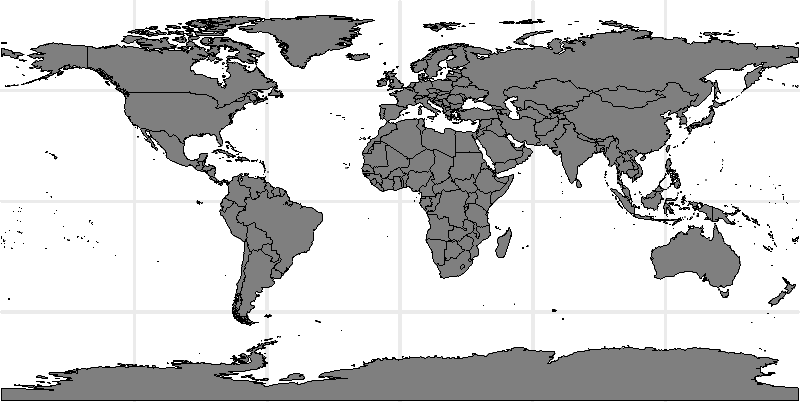
\includegraphics[keepaspectratio]{Thesis-Vayloyan6_files/figure-latex/fig-worldmap-selected-1.pdf}}
\caption{\label{fig:fig-worldmap-selected}Map Showing Countries With Available Cryptocurrency Adoption Data}
\end{figure}

\FloatBarrier

\newpage

\section{Underlying Data}\label{underlying-data}

This section discusses the underlying data used for the paper.

\subsection{Dependent Variable: Bitcoin Adoption}\label{dependent-variable-bitcoin-adoption}

Bitcoin adoption is measured using a newly released dataset by Statista (\citeproc{ref-statista_adoption}{2024b}). The dataset is the results of a survey where respondents were asked if they had used cryptocurrency in the given year. The data's first few rows can be seen in Table \ref{tab:Adoption} below. Due to the unavailability of data for the other variables for the year 2024, only data up to 2023 will be used from this set. The data is available for 56 countries of different levels of economic development.

The data quality of the survey leaves little room practical room for improvement. While survey was not representative and voluntary, opening the data quality up to self - selection issues, the only real improvement could have been a mandatory national census. The authors describe their approach to data collection and it is clear and professional: sample sizes of at least 2k people per country, checks for bots and speed racers through in the survey and the survey was performed in the official languages of the country (\citeproc{ref-statista2020}{Statista, 2020}).

\begin{table}[!h]
\centering
\caption{\label{tab:Adoption}Statista (2024a) Data: \ Share (Percentage) of Respondents Who Reported Using Cryptocurrency in Select Years}
\centering
\begin{tabular}[t]{l|r|r|r|r|r|r}
\hline
Country & 2019 & 2020 & 2021 & 2022 & 2023 & 2024\\
\hline
ARG & 16 & 14 & 21 & 35 & 26 & 30\\
\hline
AUS & 7 & 8 & 9 & 16 & 17 & 16\\
\hline
AUT & 8 & 7 & 8 & 14 & 14 & 14\\
\hline
BEL & 7 & 6 & 10 & 15 & 16 & 15\\
\hline
BRA & 18 & 12 & 12 & 22 & 28 & 24\\
\hline
CAN & 4 & 6 & 6 & 14 & 13 & 13\\
\hline
\end{tabular}
\end{table}

\subsection{Predictors: Independent and Control Variables}\label{predictors-independent-and-control-variables}

Table \ref{tab:datatable} shows an overview of the indicators used as Proxies and their sources. The indicators for currency stability, investment, wealth, remittances and risk of sovereign default are self-explanatory and should b

\begin{table}[!h]
\centering
\caption{\label{tab:datatbl}Overview of Data Sources for Independent Variables \label{tab:datatable}}
\centering
\begin{tabular}[t]{l|l|l}
\hline
Indicator & Proxy for & (Primary) Source\\
\hline
Inflation, consumer prices (annual \%) & Currency Stability & World Bank (2024c)\\
\hline
Gross domestic savings (\% of GDP) & Investment & World Bank (2024b)\\
\hline
GDP per capita (current US\$) & Wealth & World Bank (2024a)\\
\hline
Personal remittances, received (\% of GDP) & Remittances & World Bank (2024d)\\
\hline
External Debt (\% of GDP) & Risk of Sovereign Default & Focus Economics (2024)\\
\hline
Political Corruption Index (see below) & Sins & V-Dem (2024)\\
\hline
Bespoke Capital Controls Index (see below) & Capital Controls & IMF (2024)\\
\hline
\end{tabular}
\end{table}

The following proxies must be additionally discussed: Investment, Sins, Capital Controls

\textbf{Investment}

Investment is related to Savings in National Accounting, more closely in some, than in other models. In the classical view of a closed economy without government spending, savings are equal to planned investment (\citeproc{ref-mitchell2019}{Mitchell et al., 2019}). This make national savings as a percentage of GDP a good proxy for available investment funds.

\textbf{Sins}

A single indicator is used to encompass all of the Sinful uses of Bitcoin. The two primary sinful uses are criminality and the evasion of sanctions. Since Western countries routinely sanction individuals and not the countries themselves based on corruption, human rights abuses and other serious accusations, it makes sense to use corruption as a proxy for individual sanctions that people may attempt to circumvent using Bitcoin (\citeproc{ref-u.s.departmentofthetreasury2022}{U. S. Department of the Treasury, 2022}). Using corruption as a proxy for crime is also a possible approach as the link between corruption and (in particular organized) crime as been shown several regions in several studies (\citeproc{ref-buscaglia2003}{Buscaglia \& Dijk, 2003}; \citeproc{ref-mazzitelli2007}{Mazzitelli, 2007}; \citeproc{ref-centerforthestudyofdemocracy2010}{Study of Democracy, 2010}) Therefore, the political corruption index, published by V-Dem (\citeproc{ref-politica2024}{2024}) is used in an attempt to cover both crime and the likelihood that individuals attempt to move dirty money abroad. In a study with more data quantity available it would make sense to use more granular indicators, however due to the already small data size, the trade off of including several variables for the sinning attribute identified in the literature would be too adverse on the statistical power. Therefore, the ``general'' aggregated corruption by V-Dem (\citeproc{ref-politica2024}{2024}) is used, rather than one of the specific corruption indicators, for example Executive (Branch) corruption (\citeproc{ref-olin}{Olin, n.d.}).

The V-Dem (\citeproc{ref-politica2024}{2024}) data can be downloaded directly via library n R-Studio, after connecting to GitHub. To facilitate the combination with other data easier later, the world bank country codes are also added using \{countrycode\}, which can take different versions of country names and obtain the world bank code (ISO 3). The data is available only up to and including 2023.

\textbf{Capital Controls}

Since capital controls have been identified as important in section \hyperref[capital-controls]{Capital Controls}, they must be accounted for an a model attempting to explain Bitcoin adoption. Unfortunately there is a lack of structured and recent data around this topic. The most recent dataset was created by Fernandez et al. (\citeproc{ref-fernandez2016}{2016}) and was updated with data up to 2017, who produced an index to measure the severity of capital controls. The source used here will be from the online query tool of IMF (\citeproc{ref-imf2024}{2024}) which allows the recovering of information contained in the annually published Report on Exchange Arrangements and Exchange Restrictions, specifically the 5 indicators ``Controls on Personal Payments'', ``Prior Approval'', ``Quantitative Limits'', ``Indicative Limits / Bona Fide Test'' and ``Controls on Personal Capital Transactions''. The keys limitation of this dataset is that the data is only available up to and including 2022. Techniques to deal with missing data will be used to make this dataset usable, since to my knowledge it is the best available way to account for capital controls.

The first rows of the raw data can be seen in Table \ref{tab:d} below.

\begin{table}[H]
\centering
\caption{\label{tab:d}IMF (2024) Capital Controls Dummy Data}
\centering
\resizebox{\ifdim\width>\linewidth\linewidth\else\width\fi}{!}{
\begin{tabular}[t]{>{\raggedright\arraybackslash}p{0.7cm}|>{\raggedright\arraybackslash}p{1.5cm}|>{\raggedright\arraybackslash}p{1.7cm}|>{\raggedright\arraybackslash}p{2.2cm}|>{\raggedright\arraybackslash}p{2.0cm}|>{\raggedright\arraybackslash}p{2.3cm}|>{\raggedright\arraybackslash}p{3.3cm}|>{\raggedright\arraybackslash}p{3.5cm}}
\hline
Year & IFS Code & Country & Controls Personal \ Payments & Prior \ Approval & Quantitative \ Limits & Indicative Limits / \ Bona Fide Test & Controls on Personal \ Capital Transactions\\
\hline
2019  & 512  & Afghanistan  & no  & no  & no  & no  & no \\
\hline
2019  & 914  & Albania  & no  & no  & no  & no  & no \\
\hline
2019  & 612  & Algeria  & yes  & yes  & no  & yes  & yes \\
\hline
2019  & 614  & Angola  & yes  & no  & yes  & no  & yes \\
\hline
2019  & 311  & Antigua and Barbuda  & yes  & yes  & yes  & yes  & NA\\
\hline
2019  & 213  & Argentina  & yes  & yes  & yes  & yes  & yes \\
\hline
\end{tabular}}
\end{table}

In order to turn this into a quantitative variable, representing the strength of capital controls, these variables will be turned into an an index from 0-1 by assigning a value of 1 for each ``yes'' and 0 for each ``no'' and then dividing the result by the number of available data points for that country in that year, conceptually, this means that an index calculated with just one available data point look the same as one with all data points available. Additionally, it should be noted, by using an equally weighted index generating method, the (implicit) assumption is made that each of these types of restrictions is equally important in the types of capital controls that influence the adoption of cryptocurrency. In the case that a country and year has no data point (only 1 example in the data), a NA is assigned to this value. Table \ref{tab:tbl-ind-head-CC} shows the top rows of the resulting dataframe.

\begin{table}

\caption{\label{tab:tbl-ind-head-CC}Head of Table with Capital Controls Index}
\centering
\begin{tabular}[t]{l|r|r|r|r|l}
\hline
Country & 2019  & 2020  & 2021  & 2022  & 2023\\
\hline
AFG & 0.0 & 0.0 & 0.0 & 0.0 & NA\\
\hline
ALB & 0.0 & 0.0 & 0.0 & 0.0 & NA\\
\hline
DZA & 0.8 & 0.8 & 0.8 & 0.8 & NA\\
\hline
AGO & 0.6 & 0.6 & 0.6 & 0.6 & NA\\
\hline
ARG & 1.0 & 1.0 & 1.0 & 1.0 & NA\\
\hline
ARM & 0.0 & 0.0 & 0.2 & 0.2 & NA\\
\hline
\end{tabular}
\end{table}

\subsection{Data Preparation}\label{data-preparation}

This section discusses how the data is treated to prepare it for analysis.

\subsubsection{\texorpdfstring{Removing Countries not in \emph{d.Adoption}}{Removing Countries not in d.Adoption}}\label{removing-countries-not-in-d.adoption}

Countries without a dependent variable are removed in this step, since without a dependent variable nothing of insight can be gained, even if all the dependent variables are there. Due to lacking independent variable data, the value for Taiwan is also removed.

\subsubsection{\texorpdfstring{Removing Year 2024 from \emph{d.Adoption}}{Removing Year 2024 from d.Adoption}}\label{removing-year-2024-from-d.adoption}

Since there is no data for any of the other indicators for the year 2024 in a structured and accessible format, the year 2024 is removed from \emph{d.Adoption}. As entire columns of data would be missing, there is no way to sensibly impute them and get the required variance.

\subsubsection{Manually Adding Missing Data}\label{manually-adding-missing-data}

Due to the already small data size, where possible, missing independent variables are filled in manually. The following information was added in this manner. While this approach is not consistent throughout and therefore limits practical replicability, it offers the benefit of retaining slightly increased data quantity.

\begin{itemize}
\item
  Argentina Inflation Rate 2018-2022 (\citeproc{ref-statistaArgentinaInflation}{Statista, 2024a})
\item
  Nigeria Gross Domestic Savings (\% of GDP) 2018-2021 (\citeproc{ref-nigeria}{Trading Economics, 2024})
\item
  Belgium, Canada, France, Ireland, Spain External Debt (\% of GDP) 2018-2023 (\citeproc{ref-ceicdata2025}{CEIC Data, 2025})
\end{itemize}

\subsubsection{Missing Data Structure}\label{missing-data-structure}

Since not all data can be added manually due to lacking reliable and consistent data sources, alternative techniques must be employed. The type of way that missing values are dealt with depends on the quantity and structure of missing data. A standard approach is to say that any dataset having less than 5\% missing can be treated with univariate imputation, such as adding the mean of a row or column for a missing piece of data. However, the structure of the missing data plays a role too. For this reason a Missing Completely at Random (MCAR) is performed (\citeproc{ref-schwarz2024}{Schwarz, 2024}). Table \ref{tab:tblMCAR} below shows the result of this test. The results indicate that univariate imputation can be used for all variables since the hypothesis, that the data is not MCAR is either rejected at the 5\% level or the number of missing values is less than 5\%. The percentage missing applies only to the numeric columns, so the inclusion of country names in the table do not skew downwards the proportion of missing numbers.

\begin{table}[!h]
\centering
\caption{\label{tab:tblMCAR}MCAR Test Results}
\centering
\resizebox{\ifdim\width>\linewidth\linewidth\else\width\fi}{!}{
\begin{tabular}[t]{lllll>{\raggedright\arraybackslash}p{4cm}>{\raggedright\arraybackslash}p{5cm}}
\toprule
Dataset & Test Statistic & Degrees of Freedom & P-Value & Missing Patterns & Proportion Missing (\%) & Significance Level\\
\midrule
d.Adoption & 16.75 & 17 & 0.4713 & 5 & 9.45 & Not significant\\
d.Inflation & 6.39 & 9 & 0.6998 & 3 & 1.09 & Not significant\\
d.GDS & 34.5 & 12 & 6e-04 & 4 & 3.64 & Highly Significant\\
d.GDP & - & -                 No & Missing & Values & 0.00 & -\\
d.RR & 2.95 & 1 & 0.0861 & 2 & 1.82 & Not significant\\
\addlinespace
d.ED\_GDP & - & -                 No & Missing & Values & 0.00 & -\\
\bottomrule
\end{tabular}}
\end{table}

The MCAR test could not be performed for the capital controls data (\emph{d.CC}) as there is an entire column missing, as can be seen in Figure \ref{fig:md-dCC}, which is incompatible with the algorithm of the MCAR test. For this reason, in the interest of maintaining the highest reasonable data quantity, the 2022 (most recent) value of the \emph{d.CC} will be imputed in for the 2023 value of \emph{d.CC}. For a detailed guide on the interpretation of the MD Pattern figure, please see \ref{interpretation-of-missing-data-pattern-figure}.

\begin{figure}
\centering
\pandocbounded{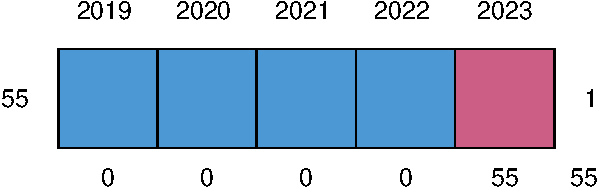
\includegraphics[keepaspectratio]{Thesis-Vayloyan6_files/figure-latex/md-dCC-1.pdf}}
\caption{\label{fig:md-dCC}Missing Pattern of d.CC}
\end{figure}

\subsubsection{Imputing Missing Data}\label{imputing-missing-data}

Since the missing data is of a structure which can use univariate imputation, this is done. The assumption behind the way that the imputations are done is that the country in which an observation happens is more important than the year in which it happens. This it is preferred to impute using the country's available data over the year's available data. Due to this dataset taking place during the Covid-19 pandemic, it would not be suitable to just take a mean of all available years for a country. Instead, the average of the year before and after the missing data is used. If a datapoint is missing in the last year, only the previous \ul{available} year's data from that country is used. If a data point is missing in the first year, only the first \ul{available} year's data point of that country is used to impute. As can be seen in Figures \ref{fig:md-Adoption} through Figure \ref{fig:md-ED-GDP} in \ref{appendix-2-missing-data-patterns}, there are many cases where the missing pattern is not in between available data points and will rely on a single imputation. For the sake of brevity, this process is referred to as Nearest Average Imputation.

To be exact, the following imputations imputations are performed:

\begin{itemize}
\item
  \emph{d.Adoption} completed using Nearest Average Imputation.
\item
  \emph{d.Inflation} completed using Nearest Average Imputation.
\item
  \emph{d.GDS} completed using Nearest Average Imputation.
\item
  No imputations required for \emph{d.GDP} (complete data).
\item
  No imputations required for \emph{d.Corruption} (complete data).
\item
  Average for all observations, divided by year, imputed for 1 country value in \emph{d.RR}, as there were no values for any year for that country United Arab Emirates. No other imputations had to be applied.
\item
  No imputations required for \emph{d.CC.}
\item
  No imputations required for \emph{d.ED\_GDP.}
\end{itemize}

With those changes, the data is ready for analysis. Please note, practically all datasets are ran through the algorithm and renamed with an ``\_imp'' suffix.

\subsubsection{Interpretation of Missing Data Pattern Figure}\label{interpretation-of-missing-data-pattern-figure}

The figure consists of horizontal bars, one for each of the configurations of missing data. Where blue represents a present year and red an absent year. The top headings represent the row headings. The number to the left of each bar represents the number of times a configuration of missing data is represented in the dataset. The number on the right represents the number of missing data points in a single observation, for a particular configuration of missing data. The number at the bottom represents the number of times a feature is missing across the dataset. The number at the bottom right represents the total number of missing variables for each dataset.

\newpage

\section{Exploratory Data Analysis}\label{exploratory-data-analysis}

This section makes exploratory analysis of the data to both understand descriptive statics and to prepare for inferential statistics by checking if assumptions for certain models are met. Please note, this entire section is performed on the imputed data.

\subsection{Box and Whisker Plots and Histograms}\label{box-and-whisker-plots-and-histograms}

The Box and Whisker Plots show not only summary statistics like the median, Interquartile Range (IQR) and outliers for each variable graphically, the separating the plots across years, changes can easily be interpreted visually. The plots show that generally, the data is close to normally distributed with either a right skew or outliers on the right. The presence of this type of structure implies a log-transformation could be applied to improve the fit in statistical models assuming normally distributed data.

\textbf{Adoption Data}

Figure \ref{fig:bw-Adoption} shows the distribution using a Box and Whisker plot of the cryptocurrency adoption data over the period studied. There seems to be an upwards trend in the median of the adoption of cryptocurrency in the available year. At the same, the number of extreme outliers peaked in 2021 and 2022, with only one country having more than 36\% adoption in 2023. The distribution is approach normal, but long-tailed on the right due to the outliers at the upper end of the range. Figure \ref{fig:hist-Adoption} further confirms the distribution approaches normal with a long rail tail. While there does appear to be a bimodal distribution for the year 2019, when looking at a histogram of all the years together (not shown), this is not the case.

\FloatBarrier

\begin{figure}
\centering
\pandocbounded{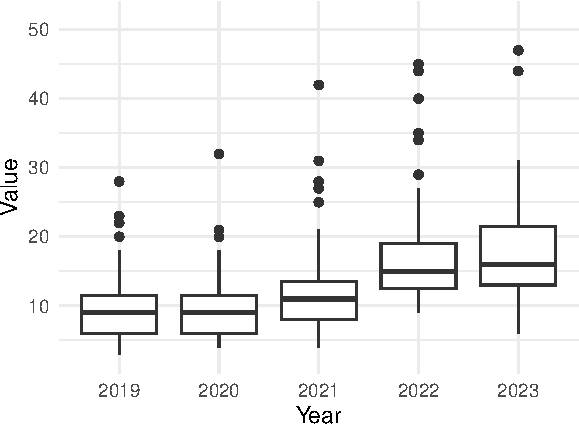
\includegraphics[keepaspectratio]{Thesis-Vayloyan6_files/figure-latex/bw-Adoption-1.pdf}}
\caption{\label{fig:bw-Adoption}Box and Whisker Plots for d.Adoption}
\end{figure}

\begin{figure}
\centering
\pandocbounded{\includegraphics[keepaspectratio]{Thesis-Vayloyan6_files/figure-latex/hist-Adoption-1.pdf}}
\caption{\label{fig:hist-Adoption}Histograms for d.Adoption}
\end{figure}

\FloatBarrier
\clearpage

\textbf{Inflation}

Figure \ref{fig:bw-Inflation} shows that the global inflation slightly increased over the period of the study until 2022 and then decreased in the final year. Due to the small size of the box and whisker plots, the distribution is hard to determine. Figure \ref{fig:hist-inf} provides histograms, which allow the right skew in the data to be seen.

\FloatBarrier

\begin{figure}
\centering
\pandocbounded{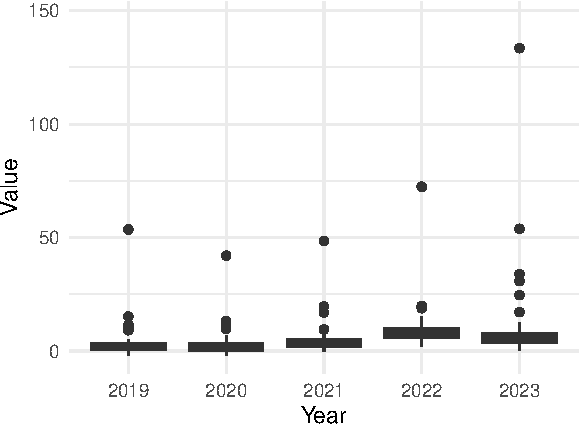
\includegraphics[keepaspectratio]{Thesis-Vayloyan6_files/figure-latex/bw-Inflation-1.pdf}}
\caption{\label{fig:bw-Inflation}Box and Whisker Plots for d.Inflation}
\end{figure}

\FloatBarrier

\begin{figure}
\centering
\pandocbounded{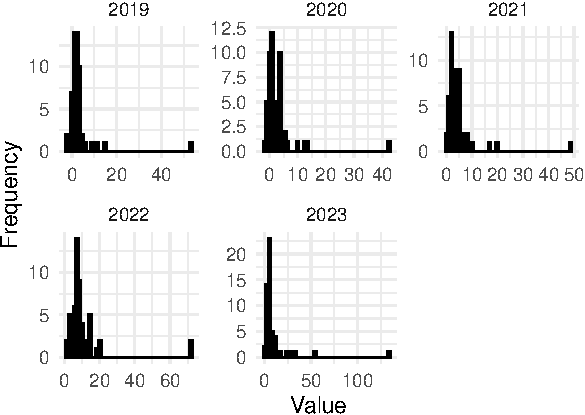
\includegraphics[keepaspectratio]{Thesis-Vayloyan6_files/figure-latex/hist-inf-1.pdf}}
\caption{\label{fig:hist-inf}Histograms for d.Inflation}
\end{figure}

\FloatBarrier
\clearpage

\textbf{Gross Domestic Savings}

Figure \ref{fig:bw-GDS} shows that the median, outliers, and distribution of Gross Domestic Savings (\% of GDP) across the studied countries remained similar throughout the period studied. With the exception of very limited outliers, the data follows a distribution approaching normal. This is confirmed by the histograms in Figure \ref{fig:hist-GDS}.

\FloatBarrier

\begin{figure}
\centering
\pandocbounded{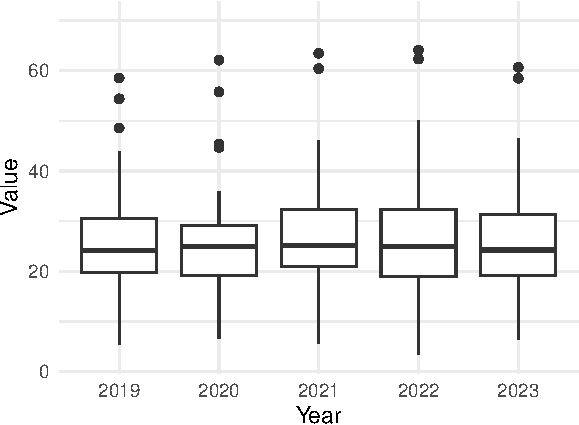
\includegraphics[keepaspectratio]{Thesis-Vayloyan6_files/figure-latex/bw-GDS-1.pdf}}
\caption{\label{fig:bw-GDS}Box and Whisker Plots for d.GDS}
\end{figure}

\FloatBarrier

\begin{figure}
\centering
\pandocbounded{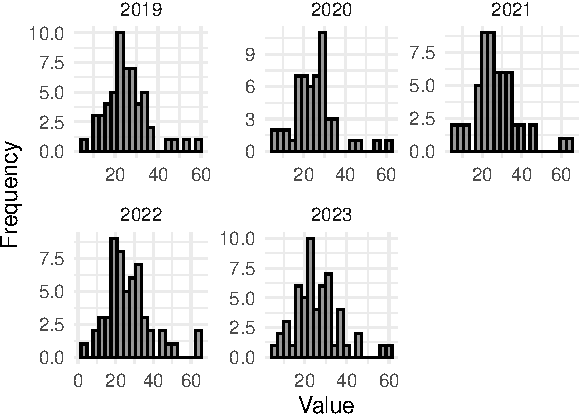
\includegraphics[keepaspectratio]{Thesis-Vayloyan6_files/figure-latex/hist-GDS-1.pdf}}
\caption{\label{fig:hist-GDS}Histograms for d.GDS}
\end{figure}

\FloatBarrier
\clearpage

\textbf{Gross Domestic Product}

Figure \ref{fig:bw-GDP} shows that, similarly to the proxy for investment, the proxy for wealth remained similar in structure throughout the time period. However, there are two key differences. In the wealth proxy, there are no outliers above 1.5 times the IQR. A second difference, which can be seen in Figure \ref{fig:hist-GDP}, is that the distribution is twin-peaked for all years except 2023.

\FloatBarrier

\begin{figure}
\centering
\pandocbounded{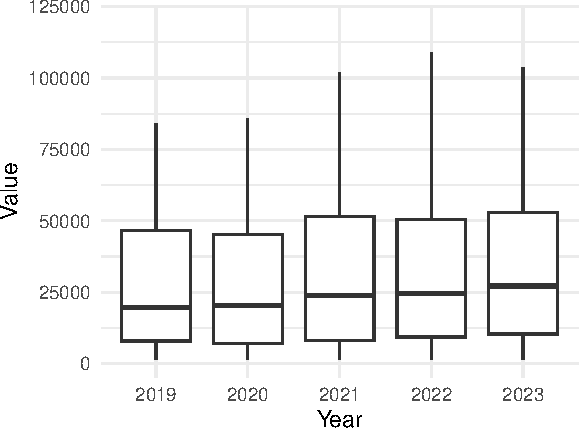
\includegraphics[keepaspectratio]{Thesis-Vayloyan6_files/figure-latex/bw-GDP-1.pdf}}
\caption{\label{fig:bw-GDP}Box and Whisker Plots for d.GDP}
\end{figure}

\FloatBarrier

\begin{figure}
\centering
\pandocbounded{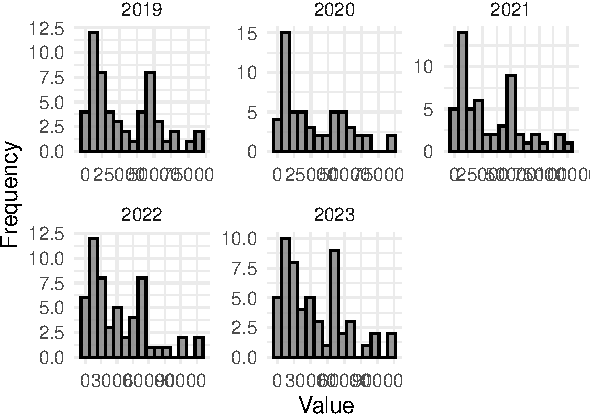
\includegraphics[keepaspectratio]{Thesis-Vayloyan6_files/figure-latex/hist-GDP-1.pdf}}
\caption{\label{fig:hist-GDP}Histograms for d.GDP}
\end{figure}

\FloatBarrier
\clearpage

\textbf{Corruption}

Figure \ref{fig:bw-Corruption} shows that while there are no extreme outliers in \emph{d.Corruption}, there is a right skew in the data. This is further confirmed by Figure \ref{fig:hist-Corruption}, which shows that the distribution is right skewed, with a small peak in the right skew.

\FloatBarrier

\begin{figure}
\centering
\pandocbounded{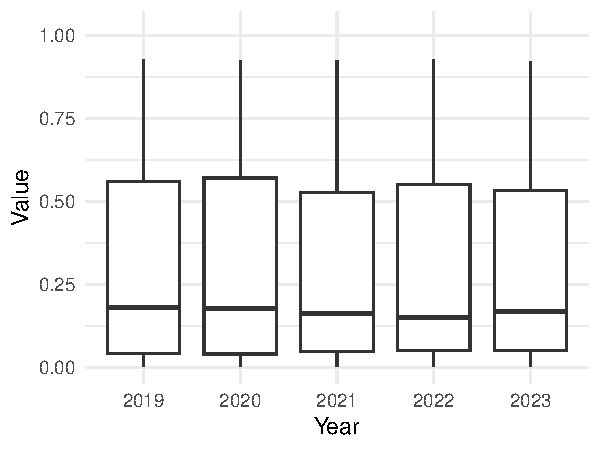
\includegraphics[keepaspectratio]{Thesis-Vayloyan6_files/figure-latex/bw-Corruption-1.pdf}}
\caption{\label{fig:bw-Corruption}Box and Whisker Plots for d.Corruption}
\end{figure}

\FloatBarrier

\begin{figure}
\centering
\pandocbounded{\includegraphics[keepaspectratio]{Thesis-Vayloyan6_files/figure-latex/hist-Corruption-1.pdf}}
\caption{\label{fig:hist-Corruption}Histograms for d.Corruption}
\end{figure}

\FloatBarrier
\clearpage

\textbf{Remittances}

Figures \ref{fig:bw-RR} and \ref{fig:hist-RR} shows that there are both outliers at the positive end of the data as well as a long tail on the right.

\FloatBarrier

\begin{figure}
\centering
\pandocbounded{\includegraphics[keepaspectratio]{Thesis-Vayloyan6_files/figure-latex/bw-RR-1.pdf}}
\caption{\label{fig:bw-RR}Box and Whisker Plots for d.RR}
\end{figure}

\FloatBarrier

\begin{figure}
\centering
\pandocbounded{\includegraphics[keepaspectratio]{Thesis-Vayloyan6_files/figure-latex/hist-RR-1.pdf}}
\caption{\label{fig:hist-RR}Histograms for d.RR}
\end{figure}

\FloatBarrier
\clearpage

\textbf{Capital Controls}

Figure \ref{fig:bw-CC} and Figure \ref{fig:hist-CC} show the distribution across years for the capital controls variable. There is a right skew.

\FloatBarrier

\begin{figure}
\centering
\pandocbounded{\includegraphics[keepaspectratio]{Thesis-Vayloyan6_files/figure-latex/bw-CC-1.pdf}}
\caption{\label{fig:bw-CC}Box and Whisker Plots for d.CC}
\end{figure}

\FloatBarrier

\begin{figure}
\centering
\pandocbounded{\includegraphics[keepaspectratio]{Thesis-Vayloyan6_files/figure-latex/hist-CC-1.pdf}}
\caption{\label{fig:hist-CC}Histograms for d.CC}
\end{figure}

\FloatBarrier
\clearpage

\textbf{External Debt to GDP}

Figure \ref{fig:bw-ED-GDP} and Figure \ref{fig:hist-ED-GDP} show that the distribution is close to normal with a long tail on the right caused by outliers.

\FloatBarrier

\begin{figure}
\centering
\pandocbounded{\includegraphics[keepaspectratio]{Thesis-Vayloyan6_files/figure-latex/bw-ED-GDP-1.pdf}}
\caption{\label{fig:bw-ED-GDP}Box and Whisker Plots for d.ED\_GDP}
\end{figure}

\FloatBarrier

\begin{figure}
\centering
\pandocbounded{\includegraphics[keepaspectratio]{Thesis-Vayloyan6_files/figure-latex/hist-ED-GDP-1.pdf}}
\caption{\label{fig:hist-ED-GDP}Histograms for d.ED\_GDP}
\end{figure}

\FloatBarrier
\clearpage

\subsection{Correlation Matrix}\label{correlation-matrix}

A correlation matrix displays visually a relationship between two continuous variables. It is important to evaluate this, since an assumption behind many some statistical models, particularily regression is that there is no \textbf{multicollinearity} (\citeproc{ref-statisticssolutions}{Statistics Solutions, n.d.}). Figure \ref{fig:corr-heatmap-show} shows a correlation heatmap for independent variables, the numbers inside of the cells (as well as their coloring, as indicated on the heatmap) shows the pearson correlation coefficient between two independent variables in the datasets. The variables associates with each correlation can be identified by looking at the row and column of that cell. The plot shows that most correlations are weak to moderate, with a median absolute value of correlations equal to 0.29 and a maximum equal to 0.79 .\footnote{The summary statistics present here were calculated without the correlation of variables with themselves (diagonal 1s in Figure \ref{fig:corr-heatmap-show})} This indicates that multicollinearity will not be a problem since even the largest absolute value is below the 0.8 threshold specified in Statistics Solutions (\citeproc{ref-statisticssolutions}{n.d.}). The diagonal values of 1 represent to correlation of each variable with itself, which is not directly relevant. Please note, each correlation is represented twice (one with a given variable on the x-axis and once on the y-axis.

\begin{figure}
\centering
\pandocbounded{\includegraphics[keepaspectratio]{Thesis-Vayloyan6_files/figure-latex/corr-heatmap-show-1.pdf}}
\caption{\label{fig:corr-heatmap-show}Correlation Heatmap of Independent Variables}
\end{figure}

\subsection{Power Transformations}\label{power-transformations}

As was seen in section \ref{exploratory-data-analysis}, there were skews in the data. Models should be considered whereby these skews are removed to present a model which has data more closely matching the assumptions of the models. To conduct transformations in a consistent and repeatable way, the \textbf{Yeo - Johnson} transformation is applied (without centering or scaling). This transformation can be thought of an extension of the Boxcox transformation, with the added benefit of working on zero and negative numbers in the dataset. Since the inflation data contains negative rates, this makes the most sense. The purpose of the transformation is to find a value \(\lambda\), which produces the optimal transformation. Where the transformation applied will be dependent on the value of the series and the \(\lambda\) itself (\citeproc{ref-featureengine}{Feature Engine, n.d.}). It is implemented here using \{caret\}. The resulting \(\lambda\) values for each variable can be seen in the table below

\[
\psi(\lambda, y) =
\begin{cases} 
\frac{(y+1)^\lambda - 1}{\lambda} & \text{if } \lambda \neq 0, y \geq 0 \\ 
\log(y+1) & \text{if } \lambda = 0, y \geq 0 \\ 
-\frac{(-y+1)^{2-\lambda} - 1}{2 - \lambda} & \text{if } \lambda \neq 2, y < 0 \\ 
-\log(-y+1) & \text{if } \lambda = 2, y < 0 
\end{cases}
\]

\begin{table}[!h]
\centering
\caption{\label{tab:YJ-Transformations-Presentation}Yeo Johnson Transformation Lambda (rounded)}
\centering
\begin{tabular}[t]{lr}
\toprule
  & x\\
\midrule
Year & 0.71\\
Adoption & -0.15\\
Inflation & 0.16\\
GDS & 0.43\\
GDP & 0.25\\
\addlinespace
Corruption & -1.56\\
RR & -0.95\\
ED_GDP & -0.16\\
\bottomrule
\end{tabular}
\end{table}

\newpage

\section{Results}\label{results}

This section discussed the statistical results of the models.

\subsection{Model 1: Linear Regression No Transformation}\label{model-1-linear-regression-no-transformation}

Linear Regression models are one of the simplest inferential statistical tools out there. Nevertheless they can provide detailed information on the relationships between variables. For the initial model, the temporal aspect (year) is modeled as continuous variable inside with it's own coefficient. As was seen in Figure \ref{fig:bw-Adoption}, the median adoption increases over the time period under observation, indicating that the effect of the year could be linear. Table \ref{tab:model1-presentation} shows the results of this model. {[}\ul{\textbf{Describe Model 1Results}}{]}.

Figure \ref{fig:model1predres} shows the scatterplot of the values predicted by the model versus the residuals.

\begin{table}[!h]
\centering
\caption{\label{tab:model1-presentation}Model 1 Summary}
\centering
\begin{tabular}[t]{lllll}
\toprule
term & estimate & std.error & statistic & p.value\\
\midrule
(Intercept) & -4383.10*** & 524.19 & -8.36 & 0.0000\\
Year & 2.17*** & 0.26 & 8.37 & 0.0000\\
Inflation & 0.14*** & 0.03 & 4.15 & 0.0000\\
GDS & 0.13*** & 0.04 & 3.05 & 0.0025\\
GDP & -0.00 & 0.00 & -0.24 & 0.8073\\
\addlinespace
Corruption & 14.65*** & 2.49 & 5.87 & 0.0000\\
RR & -0.35* & 0.20 & -1.81 & 0.0708\\
CC & -0.74 & 1.56 & -0.47 & 0.6372\\
ED\_GDP & 0.00 & 0.00 & 0.83 & 0.4051\\
\bottomrule
\end{tabular}
\end{table}

\begin{figure}
\centering
\pandocbounded{\includegraphics[keepaspectratio]{Thesis-Vayloyan6_files/figure-latex/model1predres-1.pdf}}
\caption{\label{fig:model1predres}Model 1: Scatterplot Showing Predicted vs.~Residuals}
\end{figure}

\subsection{Model 2: Linear Regression Transformations}\label{model-2-linear-regression-transformations}

\subsection{Model 3: Fixed Effects}\label{model-3-fixed-effects}

\subsection{Model 4: Random Effects}\label{model-4-random-effects}

\newpage

\section{Discussion}\label{discussion}

\subsection{Summary Key Findings}\label{summary-key-findings}

\subsection{Comparison With Existing Literature}\label{comparison-with-existing-literature}

\subsection{Strengths of Approach}\label{strengths-of-approach}

\subsection{Weaknesses of Approach}\label{weaknesses-of-approach}

\subsection{Future Research}\label{future-research}

\subsection{Practical and Policy Implications}\label{practical-and-policy-implications}

\newpage

\section{Conclusion}\label{conclusion}

\newpage

\section{\texorpdfstring{Bibliography (APA 7\textsuperscript{th})}{Bibliography (APA 7)}}\label{bibliography-apa-7}

\phantomsection\label{refs}
\begin{CSLReferences}{1}{0}
\bibitem[\citeproctext]{ref-ajibola2021}
Ajibola, I. O., Udoette, S. U., Muhammad, R. U., \& Anigwe, J. O. (2021). Currency Substitution and Exchange Rate Volatility in Nigeria: An Autoregressive Distributed Lag Approach. \emph{Central Bank of Nigeria Journal of Applied Statistics}, \emph{11}(2), 1--28. \url{https://doi.org/10.33429/Cjas.11220.1/8}

\bibitem[\citeproctext]{ref-alnasaa2022}
Alnasaa, M., Gueorguiev, N., Honda, J., Imamoglu, E., Mauro, P., Primus, K., \& Rozhkov, D. (2022). Crypto-assets, corruption, and capital controls: Cross-country correlations. \emph{Economics Letters}, \emph{215}, 110492. \url{https://doi.org/10.1016/j.econlet.2022.110492}

\bibitem[\citeproctext]{ref-ammous2018}
Ammous, S. (2018a). Can cryptocurrencies fulfil the functions of money? \emph{The Quarterly Review of Economics and Finance}, \emph{70}, 38--51. \url{https://doi.org/10.1016/j.qref.2018.05.010}

\bibitem[\citeproctext]{ref-ammousBTCstd}
Ammous, S. (2018b). \emph{The Bitcoin Standard: The Decentralized Alternative to Central Banking}. John Wiley \& Sons. \url{https://cryptache.ro/wp-content/uploads/2021/04/The-Bitcoin-Standard-The-Decentralized-Alternative-to-Central-Banking-PDF-Room.pdf}

\bibitem[\citeproctext]{ref-basher2022}
Basher, S. A., \& Sadorsky, P. (2022). Forecasting Bitcoin price direction with random forests: How important are interest rates, inflation, and market volatility? \emph{Machine Learning with Applications}, \emph{9}, 100355. \url{https://doi.org/10.1016/j.mlwa.2022.100355}

\bibitem[\citeproctext]{ref-baughman2022}
Baughman, G., Carapella, F., Gerszten, J., \& Mills, D. (2022). \emph{The stable in stablecoins}. \url{https://www.federalreserve.gov/econres/notes/feds-notes/the-stable-in-stablecoins-20221216.html}

\bibitem[\citeproctext]{ref-baur2021}
Baur, D. G., \& Hoang, L. T. (2021). A crypto safe haven against Bitcoin. \emph{Finance Research Letters}, \emph{38}, 101431. \url{https://doi.org/10.1016/j.frl.2020.101431}

\bibitem[\citeproctext]{ref-bbc2021}
BBC. (2021). Bitcoin: El salvador makes cryptocurrency legal tender. \emph{BBC}. \url{https://www.bbc.com/news/world-latin-america-57398274}

\bibitem[\citeproctext]{ref-berg2000}
Berg, A., \& Borensztein, E. (2000). \emph{The dollarization debate}.

\bibitem[\citeproctext]{ref-buscaglia2003}
Buscaglia, E., \& Dijk, J. van. (2003). Controlling Organized Crime and Corruption in the Public Sector. \emph{Forum on Crime and Society}, \emph{3}. \url{https://www.unodc.org/pdf/crime/forum/forum3_Art1.pdf}

\bibitem[\citeproctext]{ref-calvo2002}
Calvo, G. A. (2002). On dollarization. \emph{Economics of Transition}, \emph{10}(2), 393--403. \url{https://doi.org/10.1111/1468-0351.00117}

\bibitem[\citeproctext]{ref-carlson2016}
Carlson, J. (2016). Cryptocurrency and capital controls. \emph{SSRN}.

\bibitem[\citeproctext]{ref-catalini2022}
Catalini, C., Gortari, A. de, \& Shah, N. (2022). Some Simple Economics of Stablecoins. \emph{Annual Review of Financial Economics}, 117--135.

\bibitem[\citeproctext]{ref-ceicdata2025}
CEIC Data. (2025). \emph{External debt:} \url{https://www.ceicdata.com/en/indicator/external-debt--of-nominal-gdp}

\bibitem[\citeproctext]{ref-centralbanknews2025}
Central Bank News. (2025). \emph{Inflation Targets}. \url{http://www.centralbanknews.info/p/inflation-targets.html}

\bibitem[\citeproctext]{ref-chainalysis2020}
Chainalysis. (2020). \emph{The 2020 global crypto adopption index: Cryptocurrency is a global phenomenon}. \url{https://blog.chainalysis.com/reports/2020-global-cryptocurrency-adoption-index-2020}

\bibitem[\citeproctext]{ref-chainalysis2024}
Chainalysis. (2024). \emph{The 2024 Geography of Crypto Report} (p. 134). \url{https://go.chainalysis.com/2024-geography-of-cryptocurrency-report.html}

\bibitem[\citeproctext]{ref-choi2022}
Choi, S., \& Shin, J. (2022). Bitcoin: An inflation hedge but not a safe haven. \emph{Finance Research Letters}, \emph{46}, 102379. \url{https://doi.org/10.1016/j.frl.2021.102379}

\bibitem[\citeproctext]{ref-conlon2021}
Conlon, T., Corbet, S., \& McGee, R. J. (2021). Inflation and cryptocurrencies revisited: A time-scale analysis. \emph{Economics Letters}, \emph{206}, 109996. \url{https://doi.org/10.1016/j.econlet.2021.109996}

\bibitem[\citeproctext]{ref-cryptodaily2025}
Cryptodaily. (2025). \emph{Abu Dhabi{'}s Sovereign Wealth Fund Discloses Substantial BTC Holdings}. \url{https://cryptodaily.co.uk/2025/02/abu-dhabis-sovereign-wealth-fund-discloses-substantial-btc-holdings}

\bibitem[\citeproctext]{ref-dyhrberg2018}
Dyhrberg, A. H., Foley, S., \& Svec, J. (2018). How investible is Bitcoin? Analyzing the liquidity and transaction costs of Bitcoin markets. \emph{Economics Letters}, \emph{171}, 140--143. \url{https://doi.org/10.1016/j.econlet.2018.07.032}

\bibitem[\citeproctext]{ref-featureengine}
Feature Engine. (n.d.). \emph{YeoJohnsonTransformer}. \url{https://feature-engine.trainindata.com/en/1.8.x/user_guide/transformation/YeoJohnsonTransformer.html}

\bibitem[\citeproctext]{ref-fernandez2016}
Fernandez, A., Klein, M., Rebucci, A., Schindler, M., \& Uribe, M. (2016). Capital control measures: A new dataset. \emph{IMF Economic Review}, \emph{64}, 548--574. \url{https://www.columbia.edu/~mu2166/fkrsu/}

\bibitem[\citeproctext]{ref-focuseconomics2024}
Focus Economics. (2024). \emph{External debt (}. \url{https://www.focus-economics.com/economic-indicator/external-debt/}

\bibitem[\citeproctext]{ref-folkinshteyn2015}
Folkinshteyn, D., Lennon, M., \& Reilly, T. (2015). \emph{The Bitcoin Mirage: An Oasis of Financial Remittance}. \emph{2}.

\bibitem[\citeproctext]{ref-gaies2024}
Gaies, B., ChaC"bane, N., Arfaoui, N., \& Sahut, J.-M. (2024). On the resilience of cryptocurrencies: A quantile-frequency analysis of bitcoin and ethereum reactions in times of inflation and financial instability. \emph{Research in International Business and Finance}, \emph{70}, 102302. \url{https://doi.org/10.1016/j.ribaf.2024.102302}

\bibitem[\citeproctext]{ref-gemini2021}
Gemini. (2021). \emph{2021 state of u.s. crypto} (p. 16). \url{https://www.gemini.com/gemini-2021-state-of-crypto-us.pdf}

\bibitem[\citeproctext]{ref-glaser2014}
Glaser, F., Zimmermann, K., Haferkorn, M., Weber, M., \& Siering, M. (2014). \emph{Twenty second european confrence on information systems}.

\bibitem[\citeproctext]{ref-guidotti1993}
Guidotti, P. E. (1993). Currency Substitution and Financial Innovation. \emph{Journal of Money, Credit and Banking}, \emph{25}(1), 109--124. \url{https://www.jstor.org/stable/pdf/2077823.pdf}

\bibitem[\citeproctext]{ref-honig2009}
Honig, A. (2009). Dollarization, exchange rate regimes and government quality. \emph{Journal of International Money and Finance}, \emph{28}(2), 198--214. \url{https://ssrn.com/abstract=305497}

\bibitem[\citeproctext]{ref-hu2021}
Hu, M., Lee, A. D., \& Putnins, T. J. (2021). Evading Capital Controls via Cryptocurrencies: Evidence from the Blockchain. \emph{SSRN Electronic Journal}. \url{https://doi.org/10.2139/ssrn.3956933}

\bibitem[\citeproctext]{ref-imf2024}
IMF. (2024). \emph{IMF AREAER database}. \url{https://www.elibrary-areaer.imf.org/Pages/ChapterQuery.aspx}

\bibitem[\citeproctext]{ref-ju}
Ju, J. (2020). The Relationship Between Currency Substitution and Exchange Rate Volatility. \emph{University of California at Berkley, Department of Economics}. https://doi.org/\url{https://econ.berkeley.edu/sites/default/files/ECON_H195B_Thesis\%20(8).pdf}

\bibitem[\citeproctext]{ref-kantonzug}
Kanton Zug. (n.d.). \emph{Tax payments with cryptocurrencies}. \url{https://zg.ch/de/steuern-finanzen/steuern/steuerbezug/taxpaymentswithcryptocurrencies}

\bibitem[\citeproctext]{ref-kokenyne2010}
Kokenyne, A., Ley, J., \& Veyrune, R. (2010). \emph{Dedollarization}.

\bibitem[\citeproctext]{ref-kosse2023}
Kosse, A., Glowka, M., Mattei, I., \& Rice, T. (2023). \emph{Will the real stablecoin please stand up?} \url{https://www.bis.org/publ/bppdf/bispap141.pdf}

\bibitem[\citeproctext]{ref-lammer2019}
Lammer, D., Hanspal, T., \& Hackethal, A. (2019). Who Are the Bitcoin Investors? Evidence from Indirect Cryptocurrency Investments. \emph{SSRN Electronic Journal}. \url{https://doi.org/10.2139/ssrn.3501549}

\bibitem[\citeproctext]{ref-levy2021}
Levy, E. (2021). \emph{Financial dollarization and de-dollarization in the new millennium}.

\bibitem[\citeproctext]{ref-lyons2020}
Lyons, R. K., \& Viswanath-Natraj, G. (2020). \emph{What Keeps Stablecoins Stable?} (p. 63). \url{https://www.nber.org/system/files/working_papers/w27136/w27136.pdf}

\bibitem[\citeproctext]{ref-macfarlane2021}
Macfarlane, E. (2021). Strengthening Sanctions: Solutions to Curtail the Evasion of International Economic Sanctions Through the Use of Cryptocurrency. \emph{Michigan Journal of International Law}, \emph{42}, 199. \url{https://doi.org/10.36642/mjil.42.1.strengthening}

\bibitem[\citeproctext]{ref-marmora2021}
Marmora, P. (2021). Currency substitution in the shadow economy: International panel evidence using local Bitcoin trade volume. \emph{Economics Letters}, \emph{205}, 109926. \url{https://doi.org/10.1016/j.econlet.2021.109926}

\bibitem[\citeproctext]{ref-mazzitelli2007}
Mazzitelli, A. L. (2007). Transnational Organized Crime in West Africa: The Additional Challenge. \emph{International Affairs}, \emph{83}(6), 1071--1090. \url{https://doi.org/10.1111/j.1468-2346.2007.00674.x}

\bibitem[\citeproctext]{ref-mcnickel2024}
McNickel, D. (2024). \emph{{"}100}. \url{https://bravenewcoin.com/insights/100-political-kill-ex-diem-ceo-on-the-death-of-metas-stablecoin}

\bibitem[\citeproctext]{ref-mitchell2019}
Mitchell, W., Wray, L. R., \& Watts, M. J. (2019). \emph{Macroeconomics}. Macmillan International Higher Education.

\bibitem[\citeproctext]{ref-olin}
Olin, M. (n.d.). \emph{Measuring Corruption in Sustainable Development Target 16.5 with V-Dem Data}. \url{https://v-dem.net/media/publications/v-dem_policybrief_13_2017.pdf}

\bibitem[\citeproctext]{ref-parino}
Parino, F., Beiro, M. G., \& Gauvin, L. (2018). \emph{Analysis of the Bitcoin blockchain: Socio-economic factors behind the adoption}.

\bibitem[\citeproctext]{ref-phochanachan2022}
Phochanachan, P., Pirabun, N., Leurcharusmee, S., \& Yamaka, W. (2022). Do Bitcoin and Traditional Financial Assets Act as an Inflation Hedge during Stable and Turbulent Markets? Evidence from High Cryptocurrency Adoption Countries. \emph{Axioms}, \emph{11}(7), 339. \url{https://doi.org/10.3390/axioms11070339}

\bibitem[\citeproctext]{ref-ruehmann2020}
RC\textless hmann, F., Konda, S. A., Horrocks, P., \& Taka, N. (2020). \emph{Can blockchain technology reduce the cost of remittances?}

\bibitem[\citeproctext]{ref-rennhack2006}
Rennhack, R., \& Nozaki, M. (2006). \emph{Financial dollarization in latin america}.

\bibitem[\citeproctext]{ref-ricci2020}
Ricci, P. (2020). How economic freedom reflects on the Bitcoin transaction network. \emph{Journal of Industrial and Business Economics}, \emph{47}(1), 133--161. \url{https://doi.org/10.1007/s40812-019-00143-9}

\bibitem[\citeproctext]{ref-ruchti}
Ruchti, A. (2019). \emph{Digital payments: Libra - the future of money}. \url{https://www.juliusbaer.com/index.php?eID=dumpFile&t=f&f=3654&token=f26beda04ac5607dd4ffa245cd4d4f9627536fee}

\bibitem[\citeproctext]{ref-sarvi2020}
Sarvi, S. (2020). Identification and ranking of the most suitable virtual currencies for selling crude oil under sanctions. \emph{P Etroleum}, \emph{4}(1).

\bibitem[\citeproctext]{ref-saurabh2017}
Saurabh, R. (2017). \emph{Primer on bitcoin}. \url{https://pahleindia.org/wp-content/uploads/2022/12/Primer-on-Bitcoin.pdf}

\bibitem[\citeproctext]{ref-schwarz2024}
Schwarz, J. (2024). \emph{Lecture 04: Missing values \& Anomaly detection}.

\bibitem[\citeproctext]{ref-sims2001}
Sims, C. A. (2001). Fiscal Consequences for Mexico of Adopting the Dollar. \emph{Journal of Money, Credit and Banking}, \emph{33}(2), 597. \url{https://doi.org/10.2307/2673918}

\bibitem[\citeproctext]{ref-smales2024}
Smales, L. A. (2024). Cryptocurrency as an alternative inflation hedge? \emph{Accounting \& Finance}, \emph{64}(2), 1589--1611. \url{https://doi.org/10.1111/acfi.13193}

\bibitem[\citeproctext]{ref-statista2020}
Statista. (2020). \emph{Global consumer survey 2020: Content \& methodology}. \url{https://www.statista.com/download/2020_Statista_Global_Consumer_Survey_Methodology_ENG.pdf}

\bibitem[\citeproctext]{ref-statistaArgentinaInflation}
Statista. (2024a). Argentina: Inflation rate from 2004 to 2029. In \emph{Statista}. \url{https://www.statista.com/statistics/316750/inflation-rate-in-argentina/}

\bibitem[\citeproctext]{ref-statista_adoption}
Statista. (2024b). \emph{Crypto ownership by country 2019-2024}. \url{https://www.statista.com/statistics/1202468/global-cryptocurrency-ownership/}

\bibitem[\citeproctext]{ref-statistaCryptoMarketCap}
Statista. (2025). Overall cryptocurrency market capitalization per week from July 2010 to January 2025. In \emph{Statista}. \url{https://www.statista.com/statistics/730876/cryptocurrency-maket-value/}

\bibitem[\citeproctext]{ref-statisticssolutions}
Statistics Solutions. (n.d.). \emph{Assumptions of multiple linear regression analysis}. \url{https://www.statisticssolutions.com/free-resources/directory-of-statistical-analyses/assumptions-of-linear-regression/}

\bibitem[\citeproctext]{ref-stix2011}
Stix, H. (2011). Euroization: What factors drive its persistence? Household data evidence for croatia, slovenia and slovakia. \emph{Applied Economics}, \emph{43}(21), 2689--2704. https://doi.org/\url{https://doi.org/10.1080/00036840903357413}

\bibitem[\citeproctext]{ref-centerforthestudyofdemocracy2010}
Study of Democracy, C. for the. (2010). \emph{Examining the links between organised crime and corruption}. \url{http://link.springer.com/10.1007/s12117-010-9113-x}

\bibitem[\citeproctext]{ref-taskinsoy}
Taskinsoy, J. (2019). \emph{Bitcoin and turkey: A good match or a perfect storm?} \url{http://dx.doi.org/10.2139/ssrn.3477849}

\bibitem[\citeproctext]{ref-tasseven2015}
Taşseven, C., Fitzsimmons, A. P., \& Elifoglu, I. H. (2015). Currency substitution in turkey: Macroeconomic determinants. \emph{Journal of Emerging Markets}, \emph{20}(1-2), 52--68. \url{https://www.researchgate.net/profile/Eduardo-Goncalves-24/publication/272747279_APPRAISING_TECHNOLOGY_INNOVATION_A_METHODOLOGICAL_PROPOSAL/links/571e5cb208aed056fa226d10/APPRAISING-TECHNOLOGY-INNOVATION-A-METHODOLOGICAL-PROPOSAL.pdf\#page=29}

\bibitem[\citeproctext]{ref-nigeria}
Trading Economics. (2024). \emph{Nigeria - gross domestic savings}. \url{https://tradingeconomics.com/nigeria/gross-domestic-savings-percent-of-gdp-wb-data.html}

\bibitem[\citeproctext]{ref-u.s.departmentofthetreasury2022}
U. S. Department of the Treasury. (2022). \emph{Treasury Sanctions Over 40 Individuals and Entities Across Nine Countries Connected to Corruption and Human Rights Abuse}. \url{https://home.treasury.gov/news/press-releases/jy1155}

\bibitem[\citeproctext]{ref-ujunwa2021}
Ujunwa, A. I., Ujunwa, A., Onah, E., Nwonye, N. G., \& Chukwunwike, O. D. (2021). Extending the determinants of currency substitution in Nigeria: Any role for financial innovation? \emph{South African Journal of Economics}, \emph{4}, 1--18. \url{https://doi.org/10.1111/saje.12300}

\bibitem[\citeproctext]{ref-politica2024}
V-Dem. (2024). \emph{Political corruption index}. \url{https://ourworldindata.org/grapher/political-corruption-index?tab=chart}

\bibitem[\citeproctext]{ref-vieira2012}
Vieira, F. A. C., Holland, M., \& Resende, M. F. (2012). Financial dollarization and systemic risks: New empirical evidence. \emph{Journal of International Money and Finance}, \emph{31}(6), 1695--1714. \url{https://doi.org/10.1016/j.jimonfin.2012.03.007}

\bibitem[\citeproctext]{ref-viglione2015}
Viglione, R. (2015). Does governance have a role in pricing? Cross-country evidence from bitcoin markets. \emph{SSRN}. \url{https://papers.ssrn.com/sol3/papers.cfm?abstract_id=2666243}

\bibitem[\citeproctext]{ref-voskobojnikov2020}
Voskobojnikov, A., Obada-Obieh, B., Huang, Y., \& Beznosov, K. (2020). \emph{Surviving the Cryptojungle: Perception and Management of Risk Among North American Cryptocurrency (Non)Users} (J. Bonneau \& N. Heninger, Eds.; Vol. 12059, pp. 595--614). Springer International Publishing. \url{http://link.springer.com/10.1007/978-3-030-51280-4_32}

\bibitem[\citeproctext]{ref-worldbank2018}
World Bank. (2018). \emph{Financial Inclusion on the Rise, But Gaps Remain, Global Findex Database Shows}. \url{https://www.worldbank.org/en/news/press-release/2018/04/19/financial-inclusion-on-the-rise-but-gaps-remain-global-findex-database-shows}

\bibitem[\citeproctext]{ref-worldbank2024_GDP}
World Bank. (2024a). \emph{GDP per capita (current US{\$})}. \url{https://data.worldbank.org/indicator/NY.GDP.PCAP.CD}

\bibitem[\citeproctext]{ref-worldbank2024}
World Bank. (2024b). \emph{Gross domestic savings (}. \url{https://data.worldbank.org/indicator/NY.GDS.TOTL.ZS}

\bibitem[\citeproctext]{ref-worldbank2024_Inflation}
World Bank. (2024c). \emph{Inflation, consumer prices (annual {\%})}. \url{https://data.worldbank.org/indicator/FP.CPI.TOTL.ZG}

\bibitem[\citeproctext]{ref-worldbank2024_RemittReceived}
World Bank. (2024d). \emph{Personal remittances, received ({\%} of GDP)}. \url{https://data.worldbank.org/indicator/BX.TRF.PWKR.DT.GD.ZS}

\end{CSLReferences}

\newpage

\section{Appendix 1: Structured List of Literature}\label{appendix-1-structured-list-of-literature}

This Appendix gives a visual overview of the two main important fields of academic literature for this paper.

\subsection{Literature Area 1: Drivers of Currency Substitution}\label{literature-area-1-drivers-of-currency-substitution}

Table \ref{tab:litreviewCS} below shows the overview of the key literature on currency substitution and in relation to this research. It is a visual representation of the text in section \ref{literature-review-currency-substitution}.

\FloatBarrier

\begin{table}[ht]
\centering
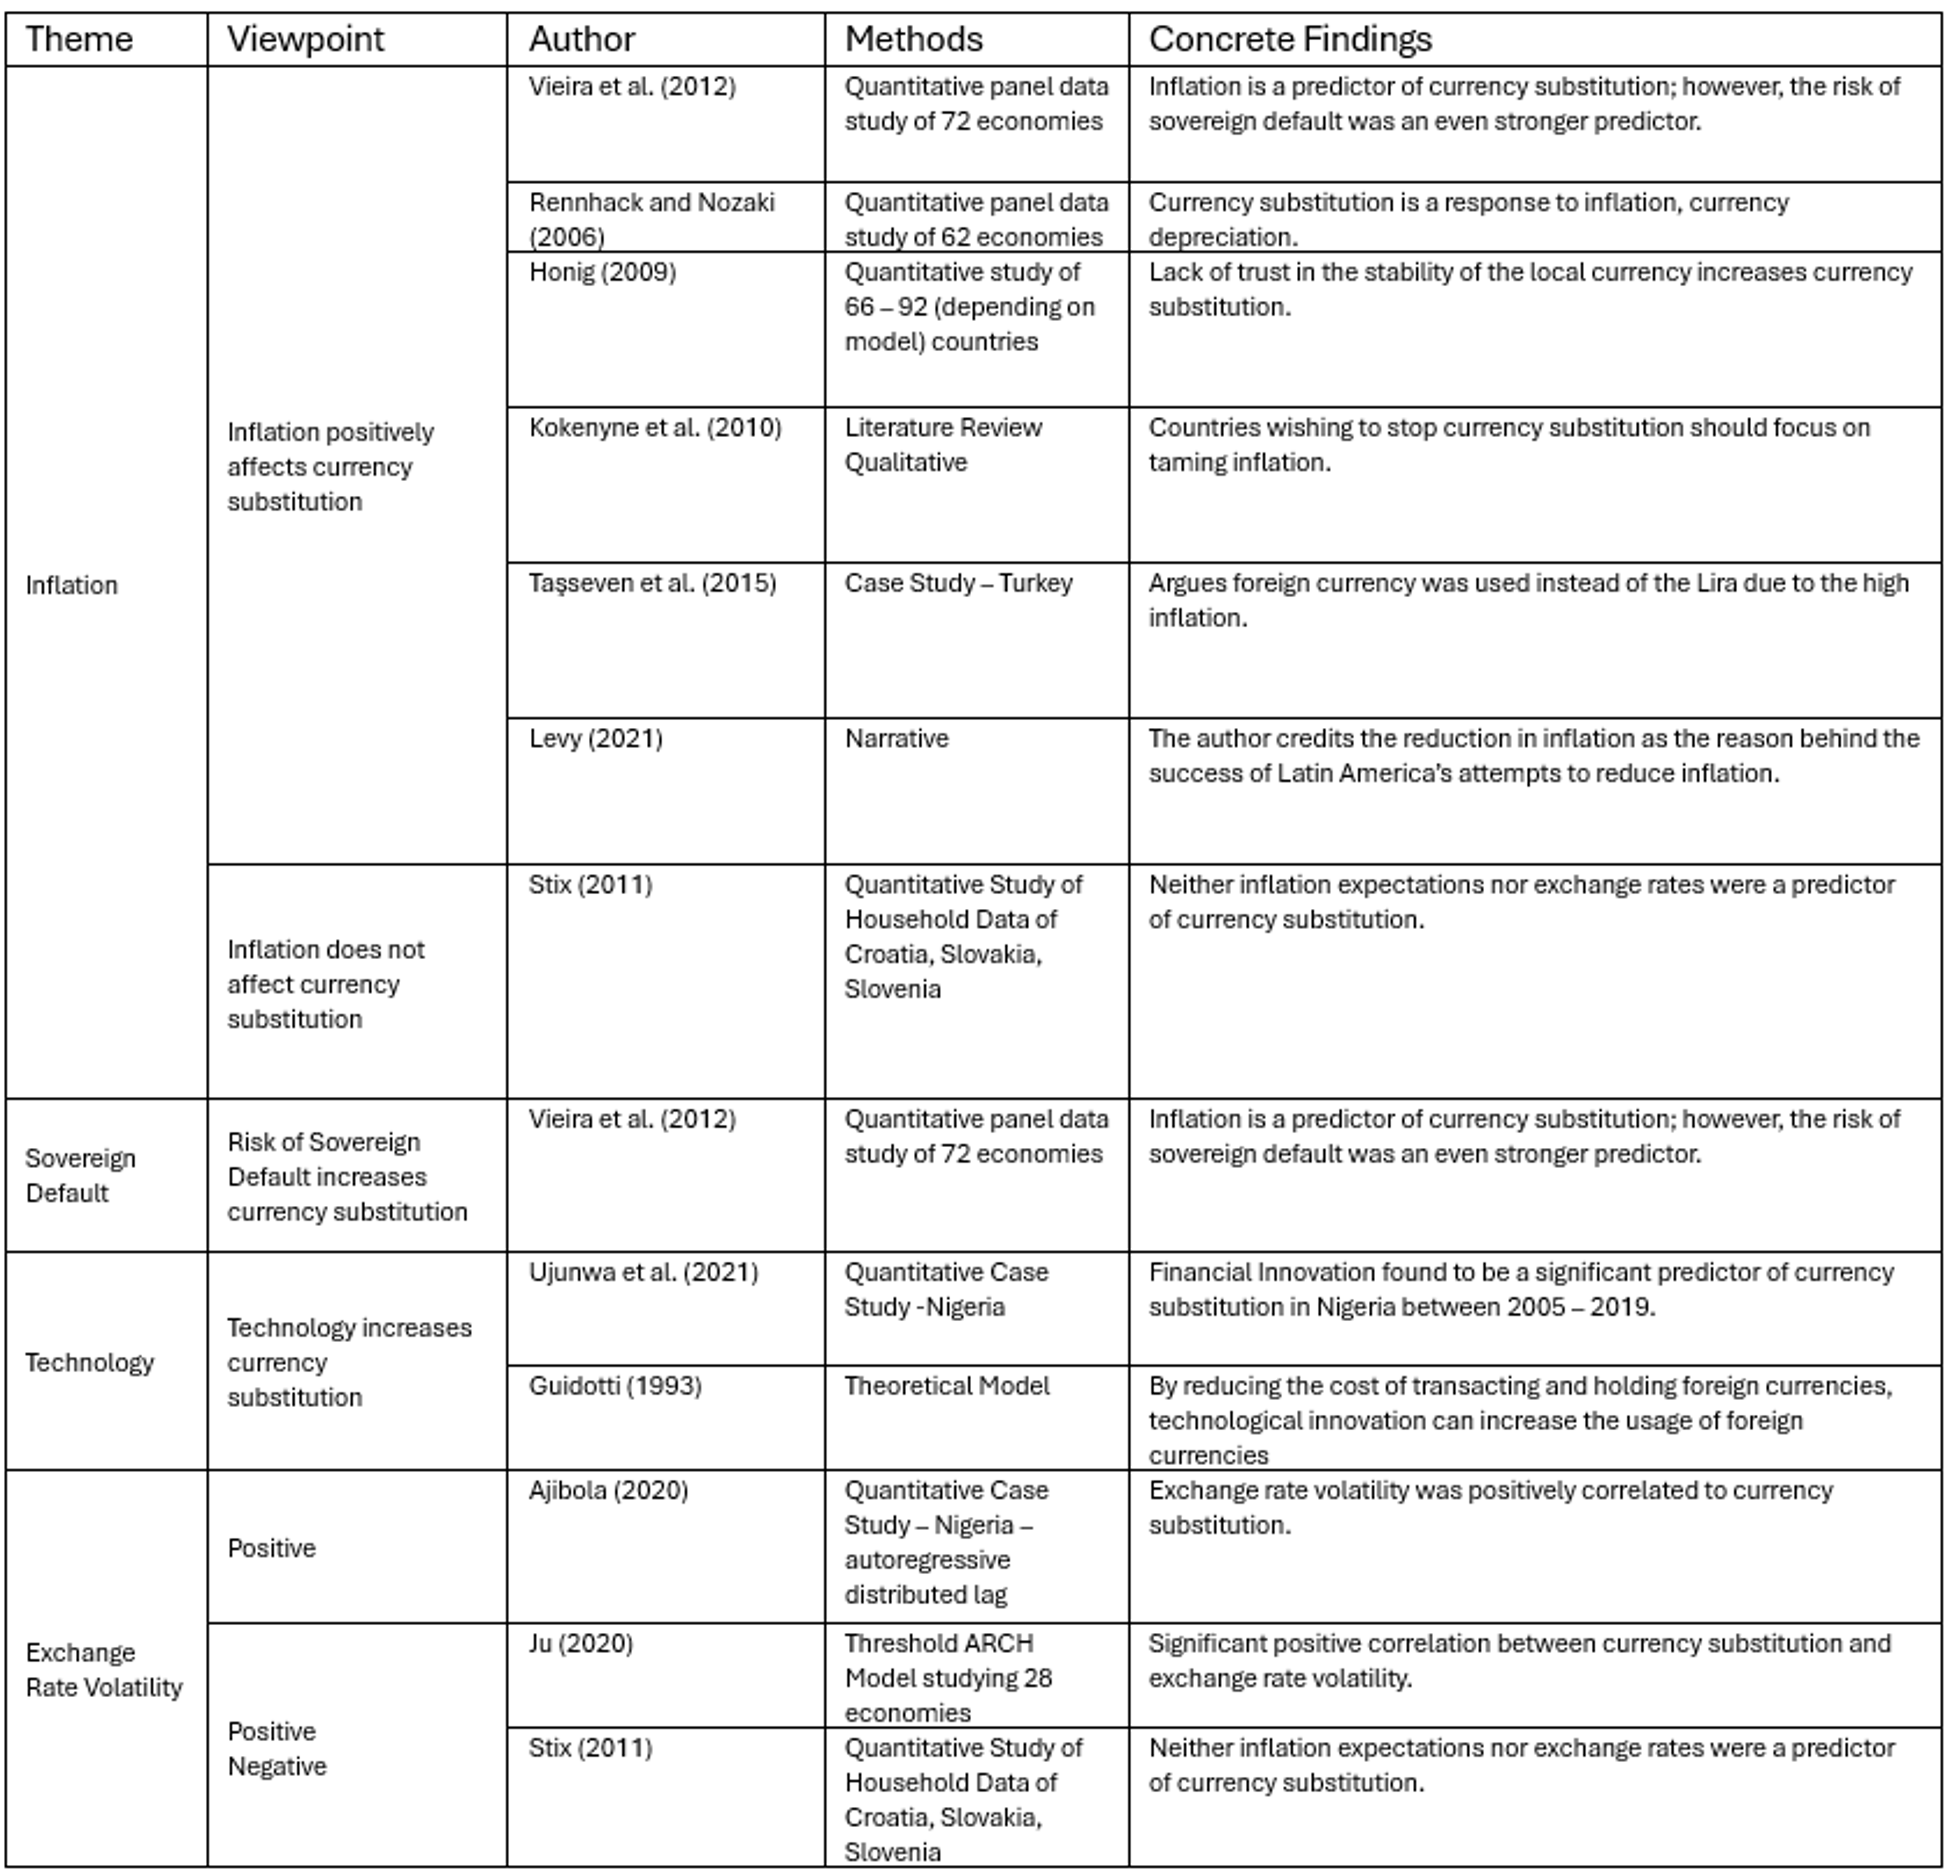
\includegraphics[width=0.9\linewidth]{review_CS.png}
\caption{Visual Summary Currency Substitution Literature}
\label{tab:litreviewCS}
\end{table}

\FloatBarrier

\newpage

\subsection{Literature Area 2: Drivers of Cryptocurrency Adoption}\label{literature-area-2-drivers-of-cryptocurrency-adoption}

Table \ref{tab:litreviewCA} below shown the overview of the key literature on the adoption of cryptocurrencies in relation to this research. It is a graphical representation of the text in section \ref{literature-review-adoption-of-cryptocurrency}

\FloatBarrier

\begin{table}[ht]
\centering
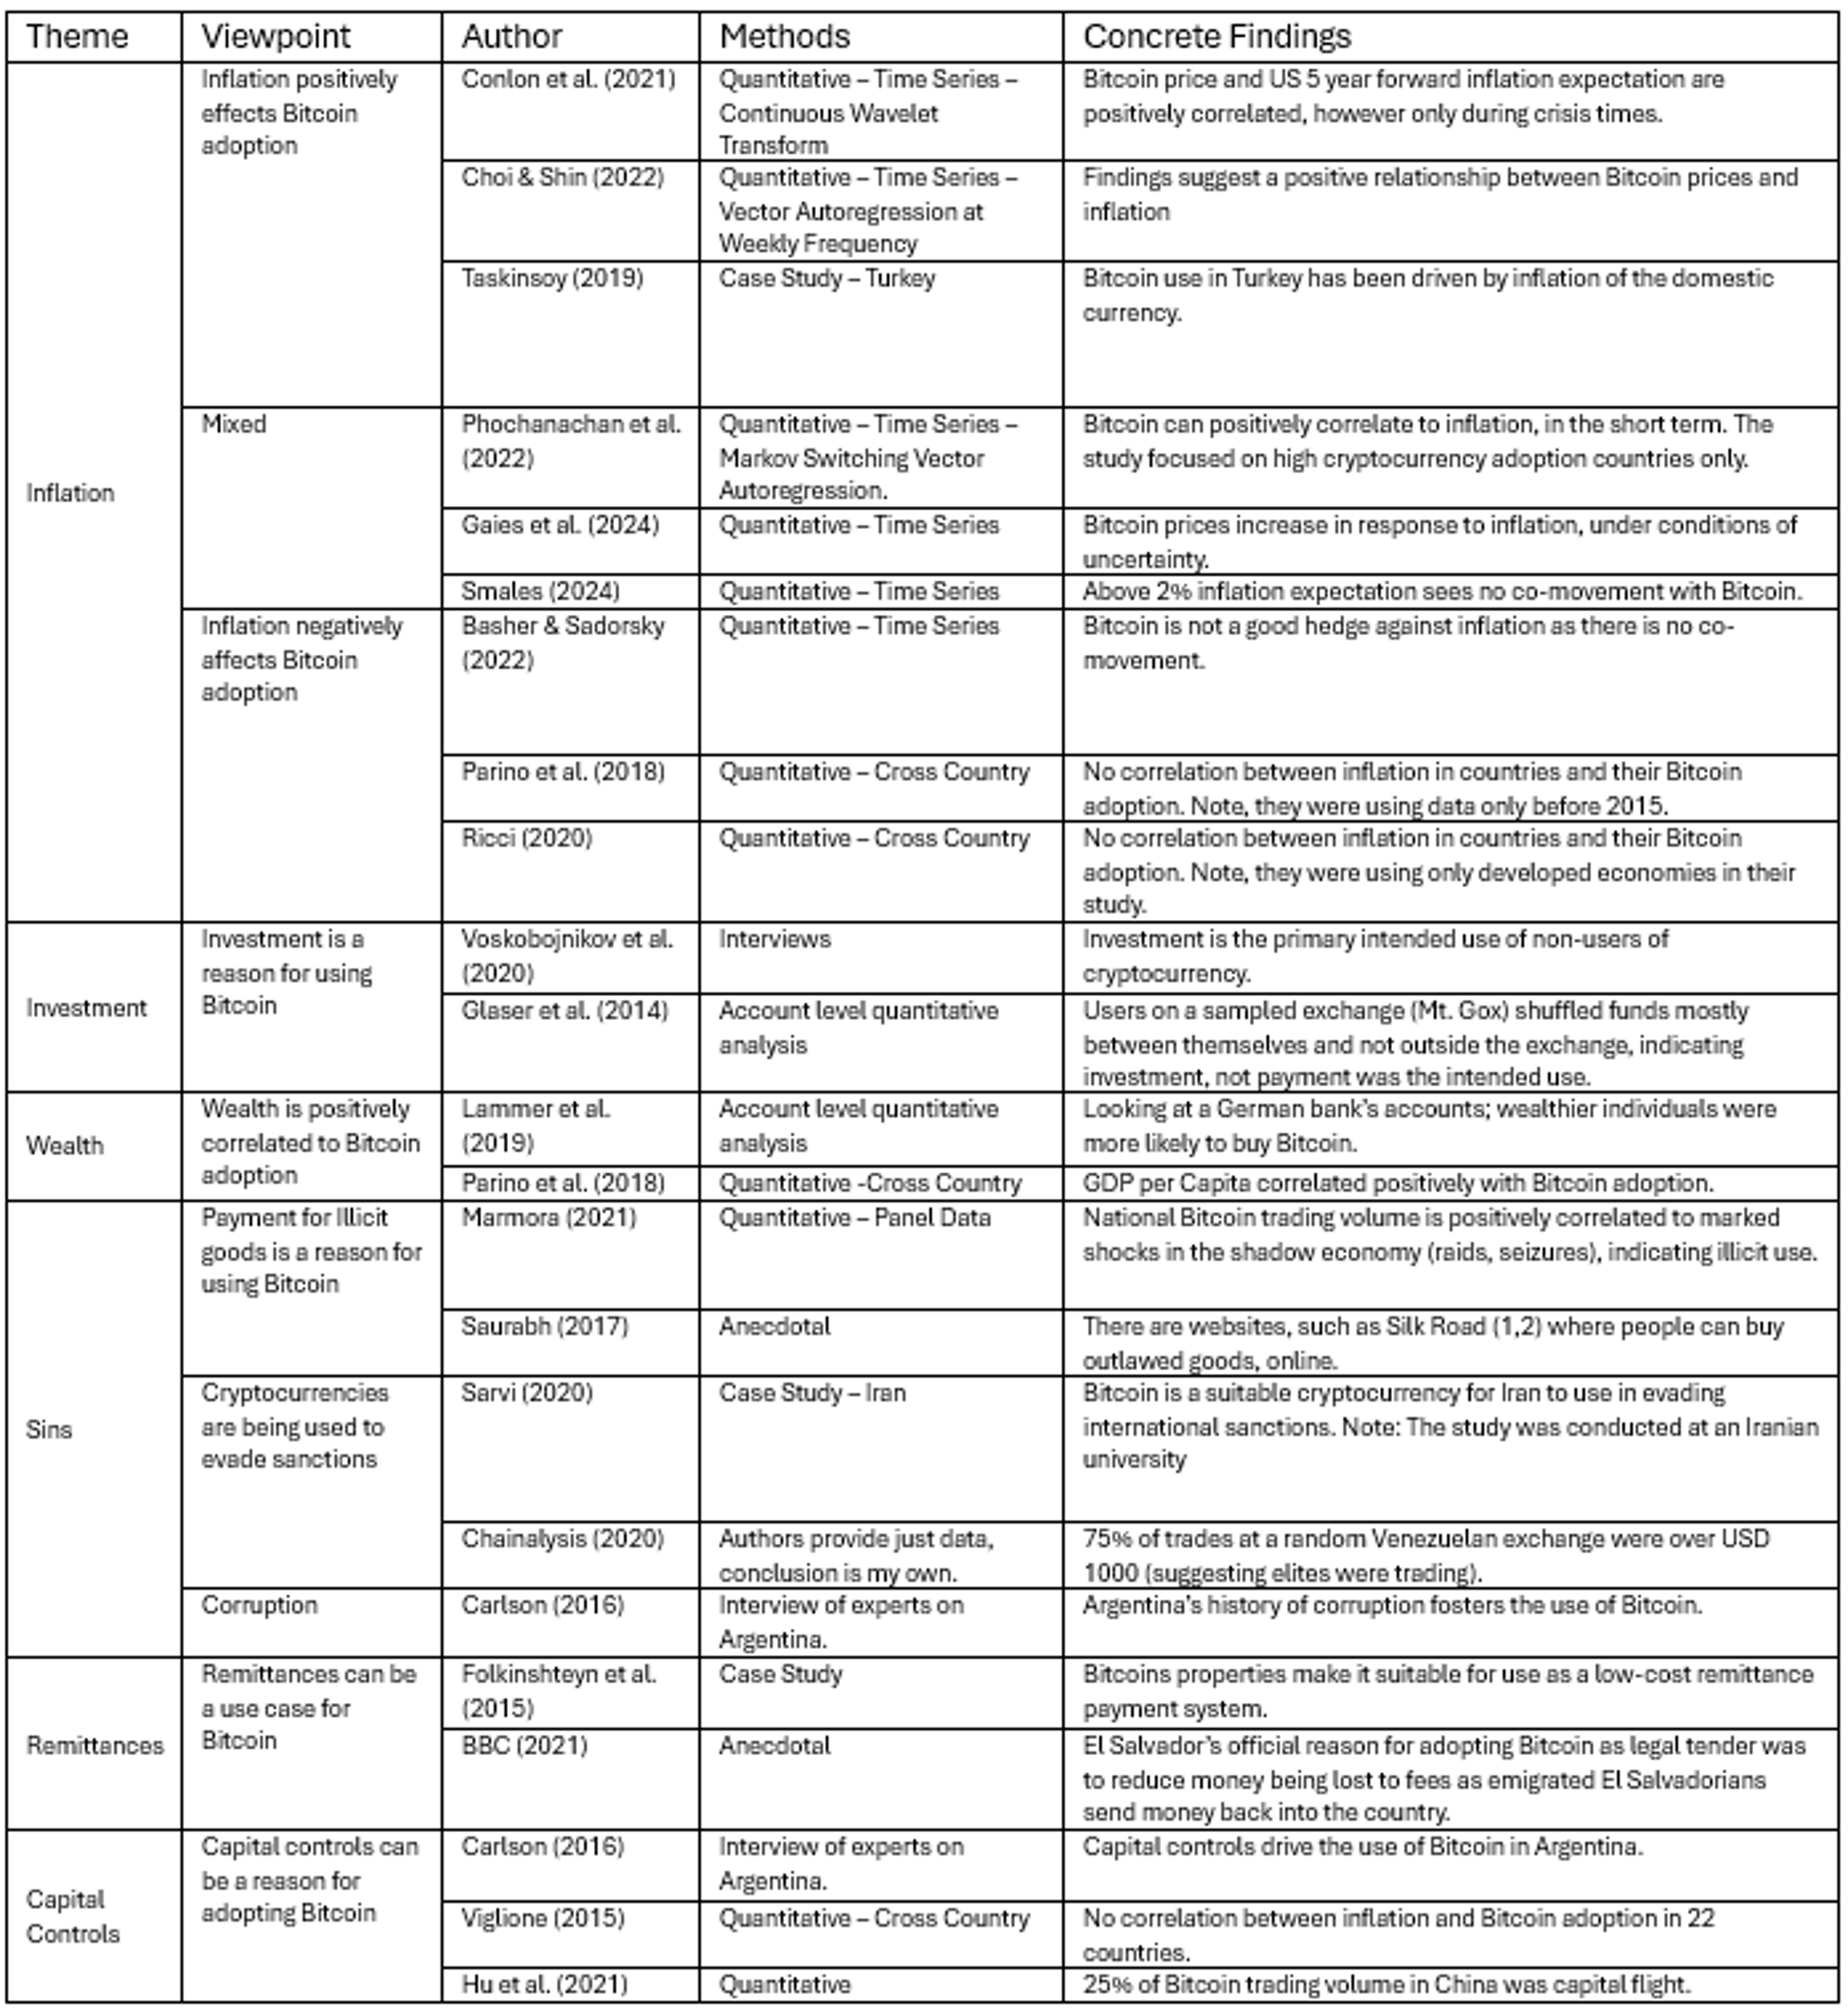
\includegraphics[width=0.9\linewidth]{review_bbtc.png}
\caption{Visual Summary Cryptocurrency Adoption Literature}
\label{tab:litreviewCA}
\end{table}

\FloatBarrier

\newpage

\section{Appendix 2: Missing Data Patterns}\label{appendix-2-missing-data-patterns}

This section shows the Missing patterns for the pre-imputation data of all variables with the exception of \emph{d.CC}, as this was already presented in the section \ref{missing-data-structure}. Please see \ref{interpretation-of-missing-data-pattern-figure} for a guide on how to interpret the figure.

\FloatBarrier

\begin{figure}
\centering
\pandocbounded{\includegraphics[keepaspectratio]{Thesis-Vayloyan6_files/figure-latex/md-Adoption-1.pdf}}
\caption{\label{fig:md-Adoption}Missing Pattern d.Adoption}
\end{figure}

\begin{figure}
\centering
\pandocbounded{\includegraphics[keepaspectratio]{Thesis-Vayloyan6_files/figure-latex/md-GDS-1.pdf}}
\caption{\label{fig:md-GDS}Missing Pattern d.GDS}
\end{figure}

\begin{figure}
\centering
\pandocbounded{\includegraphics[keepaspectratio]{Thesis-Vayloyan6_files/figure-latex/md-GDP-1.pdf}}
\caption{\label{fig:md-GDP}Missing Pattern d.GDP}
\end{figure}

\begin{figure}
\centering
\pandocbounded{\includegraphics[keepaspectratio]{Thesis-Vayloyan6_files/figure-latex/md-Corruption-1.pdf}}
\caption{\label{fig:md-Corruption}Missing Pattern d.Corruption}
\end{figure}

\begin{figure}
\centering
\pandocbounded{\includegraphics[keepaspectratio]{Thesis-Vayloyan6_files/figure-latex/md-RR-1.pdf}}
\caption{\label{fig:md-RR}Missing Pattern d.RR}
\end{figure}

\begin{figure}
\centering
\pandocbounded{\includegraphics[keepaspectratio]{Thesis-Vayloyan6_files/figure-latex/md-ED-GDP-1.pdf}}
\caption{\label{fig:md-ED-GDP}Missing Pattern d.ED\_GDP}
\end{figure}

\FloatBarrier

\clearpage

\newpage

\section{Appendix 3: AI Disclosure}\label{appendix-3-ai-disclosure}

I made extensive use of AI, particularly ChatGPT for this project. The main, but not exhaustive uses were the following:

\begin{itemize}
\item
  Spelling / Reviewing and writing drafts of sections where I needed inspiration to get started.
\item
  R Studio, Markdown and LaTex issues and code suggestions.
\item
  Scanning Long Documents for parts that I needed.
\item
  Methodology ``Research'', although I verified everything using proper academic sources.
\item
  Cover Page: Used Canva's AI Image Generation to create the cover photo.
\end{itemize}

\newpage

\section{Appendix 4: GitHub Access}\label{appendix-4-github-access}

This project and associated data can be found on the following public GitHub Repository: {[}INSERT GITHUB REPOSITORY LINK{]}

\section{Boxcox}\label{boxcox}

\begin{Shaded}
\begin{Highlighting}[]
\FunctionTok{library}\NormalTok{(MASS)}
\end{Highlighting}
\end{Shaded}

\begin{verbatim}
## Warning: package 'MASS' was built under R version 4.3.3
\end{verbatim}

\begin{verbatim}
## 
## Attaching package: 'MASS'
\end{verbatim}

\begin{verbatim}
## The following object is masked from 'package:dplyr':
## 
##     select
\end{verbatim}

\begin{Shaded}
\begin{Highlighting}[]
\CommentTok{\# Run Box{-}Cox transformation and store results}
\NormalTok{boxcox\_result }\OtherTok{\textless{}{-}} \FunctionTok{boxcox}\NormalTok{(}\FunctionTok{lm}\NormalTok{(d.panel}\SpecialCharTok{$}\NormalTok{GDS }\SpecialCharTok{\textasciitilde{}} \DecValTok{1}\NormalTok{), }\AttributeTok{lambda =} \FunctionTok{seq}\NormalTok{(}\SpecialCharTok{{-}}\DecValTok{2}\NormalTok{, }\DecValTok{2}\NormalTok{, }\FloatTok{0.1}\NormalTok{), }\AttributeTok{plotit =} \ConstantTok{TRUE}\NormalTok{)}
\end{Highlighting}
\end{Shaded}

\pandocbounded{\includegraphics[keepaspectratio]{Thesis-Vayloyan6_files/figure-latex/boxcox-1.pdf}}

\begin{Shaded}
\begin{Highlighting}[]
\CommentTok{\# Extract lambda values (x{-}axis) and log{-}likelihood values (y{-}axis)}
\NormalTok{lambda\_vals }\OtherTok{\textless{}{-}}\NormalTok{ boxcox\_result}\SpecialCharTok{$}\NormalTok{x}
\NormalTok{log\_lik\_vals }\OtherTok{\textless{}{-}}\NormalTok{ boxcox\_result}\SpecialCharTok{$}\NormalTok{y}

\CommentTok{\# Find the MLE of lambda (the one maximizing log{-}likelihood)}
\NormalTok{lambda\_mle }\OtherTok{\textless{}{-}}\NormalTok{ lambda\_vals[}\FunctionTok{which.max}\NormalTok{(log\_lik\_vals)]}

\CommentTok{\# Compute the 95\% confidence interval threshold (log{-}likelihood max {-} 0.5)}
\NormalTok{ci\_threshold }\OtherTok{\textless{}{-}} \FunctionTok{max}\NormalTok{(log\_lik\_vals) }\SpecialCharTok{{-}} \FloatTok{0.5}

\CommentTok{\# Identify lambda values that fall within the confidence interval}
\NormalTok{lambda\_ci }\OtherTok{\textless{}{-}}\NormalTok{ lambda\_vals[log\_lik\_vals }\SpecialCharTok{\textgreater{}=}\NormalTok{ ci\_threshold]}

\CommentTok{\# Compute the middle value of the confidence interval}
\NormalTok{lambda\_mid }\OtherTok{\textless{}{-}} \FunctionTok{mean}\NormalTok{(}\FunctionTok{range}\NormalTok{(lambda\_ci))}

\CommentTok{\# Print results}
\FunctionTok{cat}\NormalTok{(}\StringTok{"MLE Lambda:"}\NormalTok{, lambda\_mle, }\StringTok{"}\SpecialCharTok{\textbackslash{}n}\StringTok{"}\NormalTok{)}
\end{Highlighting}
\end{Shaded}

\begin{verbatim}
## MLE Lambda: 0.4646465
\end{verbatim}

\begin{Shaded}
\begin{Highlighting}[]
\FunctionTok{cat}\NormalTok{(}\StringTok{"95\% Confidence Interval:"}\NormalTok{, }\FunctionTok{range}\NormalTok{(lambda\_ci), }\StringTok{"}\SpecialCharTok{\textbackslash{}n}\StringTok{"}\NormalTok{)}
\end{Highlighting}
\end{Shaded}

\begin{verbatim}
## 95% Confidence Interval: 0.3838384 0.5454545
\end{verbatim}

\begin{Shaded}
\begin{Highlighting}[]
\FunctionTok{cat}\NormalTok{(}\StringTok{"Middle of Confidence Interval:"}\NormalTok{, lambda\_mid, }\StringTok{"}\SpecialCharTok{\textbackslash{}n}\StringTok{"}\NormalTok{)}
\end{Highlighting}
\end{Shaded}

\begin{verbatim}
## Middle of Confidence Interval: 0.4646465
\end{verbatim}

\begin{verbatim}
## Created from 275 samples and 9 variables
## 
## Pre-processing:
##   - ignored (1)
##   - Yeo-Johnson transformation (8)
## 
## Lambda estimates for Yeo-Johnson transformation:
## 0.71, -0.15, 0.16, 0.43, 0.25, -1.56, -0.95, -0.16
\end{verbatim}

\pandocbounded{\includegraphics[keepaspectratio]{Thesis-Vayloyan6_files/figure-latex/unnamed-chunk-7-1.pdf}}

\end{document}
